\documentclass[11pt,a4paper]{article}

% ------------------------------------------------------------------
% Standalone, self-contained working document. NOT wired into the main
% thesis.tex build and NOT meant to be dropped into 03_Content/4_Results.tex
% as-is. Covers the SECOND-generation ("v2") corpus and shared space --
% see thesis/corpus/ANALYSIS_OVERVIEW.md's "Extraction pipeline v2" section
% and thesis/03_Content/3_Methods.tex's "Revising the Extraction Pipeline"
% for why v2 exists at all. Predecessor documents
% (Geometric_Analysis_Draft/, Geometric_Analysis_Draft_v2/) cover earlier,
% still-frozen-on-disk runs and are kept for comparison.
%
% This document covers run 20260910-121710, built on a corrected shared
% space (a cited-author stop-list bug fixed, entity count 753->749; see
% the fixbox below) and adds two sections that did not exist in v2 at
% all, written directly in response to researcher feedback recorded in
% Meditations/Meditation Gaps Literature Interviews.txt: (1) a per-entity
% epistemic-status breakdown -- answering that file's own question about
% how negated/questioned entities are currently treated -- and (2) a
% cross-corpus gap analysis operationalizing that file's own framing
% ("which of the literature's regions are not occupied by the
% interviews, and the reverse", for all three corpus pairs). Per that
% same feedback, both new sections are written analysis-first: findings
% and concrete example tables, not a methodology/what-changed narrative
% (that narrative lives in thesis/03_Content/3_Methods.tex).
%
% Includes a labelled "Possible interpretations" section and a plain-
% language summary, at the researcher's explicit request -- kept visibly,
% structurally separate from the descriptive-fact sections and flagged
% throughout as provisional readings for the researcher to argue with,
% not the thesis's settled Results-chapter conclusions.
% Compile directly: pdflatex geometric_analysis_report_v3.tex
% ------------------------------------------------------------------

\usepackage[a4paper,margin=2.7cm]{geometry}
\usepackage[utf8]{inputenc}
\usepackage[T1]{fontenc}
\usepackage{graphicx}
\usepackage{booktabs}
\usepackage{longtable}
\usepackage{array}
\usepackage{xcolor}
\usepackage{enumitem}
\usepackage{caption}
\usepackage{parskip}
\usepackage[colorlinks=true,linkcolor=blue!50!black,citecolor=blue!50!black,urlcolor=blue!50!black]{hyperref}
\usepackage{titlesec}
\usepackage{tabularx}

\definecolor{noteback}{RGB}{240,240,248}
\definecolor{noteline}{RGB}{120,120,180}
\newenvironment{plainbox}[1][Note]
  {\par\vspace{6pt}\noindent{\color{noteline}\rule{\linewidth}{0.6pt}}\par\vspace{3pt}
   \noindent\small\textbf{#1.}\ \ignorespaces}
  {\par\vspace{3pt}\noindent{\color{noteline}\rule{\linewidth}{0.6pt}}\vspace{6pt}\par}

\definecolor{interpline}{RGB}{180,140,60}
\newenvironment{interpbox}[1][Possible interpretation]
  {\par\vspace{6pt}\noindent{\color{interpline}\rule{\linewidth}{0.8pt}}\par\vspace{3pt}
   \noindent\small\textcolor{interpline}{\textbf{#1.}}\ \ignorespaces}
  {\par\vspace{3pt}\noindent{\color{interpline}\rule{\linewidth}{0.8pt}}\vspace{6pt}\par}

\definecolor{fixline}{RGB}{60,140,90}
\newenvironment{fixbox}[1][What was fixed]
  {\par\vspace{6pt}\noindent{\color{fixline}\rule{\linewidth}{0.8pt}}\par\vspace{3pt}
   \noindent\small\textcolor{fixline}{\textbf{#1.}}\ \ignorespaces}
  {\par\vspace{3pt}\noindent{\color{fixline}\rule{\linewidth}{0.8pt}}\vspace{6pt}\par}

\newcommand{\jargon}[1]{\textbf{#1}}

\title{\textbf{Mapping "Cult," Third Pass: Epistemic Status and Cross-Corpus Gaps}\\[4pt]
\large Working report -- draft base material for the Results chapter,\\
with a first attempt at interpretation}
\author{Prepared for C\'elestin Meunier's thesis project}
\date{Covers run \texttt{20260910-121710}, generated 2026-09-10}

\begin{document}
\maketitle

\begin{plainbox}[How to read this document]
This is still not a finished Results chapter. Sections~\ref{sec:stages}--\ref{sec:honesty}
report numbers, not arguments. Section~\ref{sec:interpretation} is a first,
explicitly provisional pass at what these patterns \emph{might} mean, kept
structurally separate and visually marked (a tan box) throughout so a
reader can tell at a glance which sentences are geometric fact and which
are a reading of that fact the researcher is free to revise or reject.
Green boxes mark a specific, checkable methodological correction made
during this run. Sections~\ref{sec:epistemic} and~\ref{sec:crossgaps} are
new this run and, per explicit researcher feedback on the previous
report, are written analysis-first -- findings and concrete example
tables up front, with only as much mechanism as is needed to read the
table correctly (the full methodology lives in
\texttt{thesis/03\_Content/3\_Methods.tex}). Nowhere in this document is
geometric proximity treated as evidence that any group, practice, or
person \emph{is} or \emph{is not} "a cult."
\end{plainbox}

\tableofcontents

% ============================================================
\section{In short: what did this run find?}
\label{sec:short}
% ============================================================

\begin{itemize}[leftmargin=1.4em]
  \item \textbf{A second bug was found and fixed in the emergent-entity
  pipeline}, on top of the entity-extraction fix already documented in
  the previous report: the corpus's own author-citation stop-list only
  correctly matched 10 of 68 literature authors (those cited
  "Surname, First" with a comma); the other 58 (plain "First Last," no
  comma) were silently passing through as if they were the author's
  whole name, so real bare-surname citations like "Richardson,"
  "Palmer," and "Barker" were never actually filtered out of the entity
  list. Fixed; the shared space now holds \textbf{749} emergent entities
  (down from 753) and \textbf{11{,}373} total points. Full story in
  Section~\ref{sec:entities}.
  \item \textbf{New this run, directly answering a standing question}:
  how are entities/concepts currently treated when the text asserts,
  negates, or merely speculates about them? Answer: almost entirely
  undifferentiated -- only \textbf{3 of 749} entities carry \emph{any}
  mention with a known (non-"unknown") epistemic tag at all, because the
  large majority of entity mentions come from a broader extraction field
  that has no per-mention stance information to draw on in the first
  place. Section~\ref{sec:epistemic}.
  \item \textbf{New this run: a genuine cross-corpus gap analysis},
  operationalizing the researcher's own framing directly -- which of the
  literature's own regions are not occupied by the interviews, and the
  reverse, and the same for MIVILUDES against both. Two complementary
  views: a lightweight check on existing unified entity clusters (of the
  \textbf{49} clusters, \textbf{40} have zero MIVILUDES presence and
  \textbf{28} have zero interview presence, while \textbf{0} have zero
  literature presence), and a heavier check that clusters each corpus's
  own entities independently and measures geometric proximity to the
  nearest entity the other corpus mentions at all -- finding, among other
  things, that several of literature's most historically notorious named
  groups (the Manson Family, the Peoples Temple, the Moonies) sit
  further from any MIVILUDES-mentioned entity than any other literature
  cluster does. Section~\ref{sec:crossgaps}.
  \item \textbf{New this run: a per-interview extraction sanity-check
  aid}, directly answering the request for a way to manually confirm
  extraction "makes sense" at the level of a single interview -- a CSV
  and a compact one-page-per-interview PDF tracing every kept expression
  and every domain-term mention back to its resolved pooled entity (or
  the exact filter it failed). Kept as a local QA artifact, not part of
  this document or the git repository, since it embeds verbatim
  participant quotes at bulk scale. Section~\ref{sec:qa-trace}.
  \item Everything else -- corpus sizes, the shared-space construction,
  clustering/topology/Voronoi/publication-date findings -- carries over
  from the previous report with numbers refreshed against this run;
  summarised in Sections~\ref{sec:stages}--\ref{sec:pubdate} below.
\end{itemize}

% ============================================================
\section{Where the project stands}
\label{sec:stages}
% ============================================================

\subsection{Why a second pass at all}
A 100-item manual fidelity review of the first extraction pipeline
(2026-09-08) found it systematically over-inclusive: paraphrased or
mistranslated expressions, document headings and bibliography citations
extracted as though they were claims, occasional interviewer questions
mislabelled as participant statements. The pipeline (\jargon{v2}) was
rebuilt around a strict verbatim-span rule plus a second, independently-
prompted model that judges every retained candidate the way a human
reviewer would ("model-judged," never a substitute for human review).
v1's own archives and every retained run stay frozen on disk, untouched.

\subsection{Stage 1--2 -- Same three corpora, far fewer expressions}
Same underlying documents as v1 (57 scholarly works, 2 MIVILUDES
documents, 25 interview transcripts with resolved extraction); far
stricter extraction:

\begin{table}[h!]
\centering
\begin{tabular}{lrrr}
\toprule
Corpus & v1 expressions & v2 expressions & Change \\
\midrule
literature & 39{,}236 & 5{,}741 & $-85.4\%$ \\
MIVILUDES & 914 & 108 & $-88.2\%$ \\
interviews & 230 & 64 & $-72.2\%$ \\
\bottomrule
\end{tabular}
\end{table}

\subsection{Stage 3--4 -- Reference vocabularies unchanged; emergent entities, corrected twice now}
The three reference vocabularies (concept backbone, structural concepts,
ConceptNet-generalised concepts) are unchanged from v1, reused as-is.
Emergent entities have now been through two rounds of correction --
see Section~\ref{sec:entities} for the full story, including this run's
own fix.

\subsection{Stage 5 -- One shared geometric space, rebuilt}
Same pooling procedure as v1: embed everything with the same model,
standardize, PCA down to the smallest dimensionality keeping 95\% of the
variance. This run's space holds \textbf{11{,}373} points, compressed to
\textbf{393} dimensions (95.0\% variance kept) -- down from the previous
report's 11{,}377 points, entirely accounted for by the 4 cited-author
names newly excluded from the entity layer (Section~\ref{sec:entities}).

\subsection{Stage 6 -- The interview "first impression" layer: ported, not redone}
Unchanged: the 25 manually-verified interview opening-prompt exemplars
are re-projected through this run's transform rather than re-selected --
the embedding of a quote is a property of its own words, not of which
build happened to be running.

\subsection{Stage 7 -- The equal-$n$ correction still applies, at a smaller scale}
Unchanged finding: literature is still \textbf{97.09\%} of expression
points, so the same equal-$n$/equal-size corrections are still necessary
and still used, drawing 64 points per source.

\subsection{Stage 8 -- Three toolkit runs now on record}
The reusable analysis toolkit, now 14 modules (2 new this run --
\texttt{analyze\_cross\_corpus\_gaps} and the epistemic-status addition
to \texttt{build\_shared\_space}'s entity loader), was run against the
corrected 749-entity space under run \texttt{20260910-121710}, covered
by this document. The previous report (run \texttt{20260910-101829})
remains a separate, still-valid document for the numbers this run did
not change; it is not superseded so much as extended.

% ============================================================
\section{Key ideas, explained in plain language}
\label{sec:jargon}
% ============================================================

Unchanged from earlier documents -- included again so this one is
self-contained. Skip if already familiar.

\subsection{Embeddings, distance, and similarity}
An \jargon{embedding} converts a piece of text into a long list of
numbers (a \jargon{vector}, 1,024 numbers here) such that similar
meanings end up as nearby vectors. \jargon{Euclidean distance} is
ordinary straight-line distance in that many-dimensional space (smaller
= more similar). \jargon{Cosine similarity} instead measures whether two
vectors point in the same \emph{direction} from the origin, ignoring
length ($-1$ opposite, $1$ identical direction, $0$ unrelated). Both are
always reported side by side.

\subsection{Centroid, standardization, and PCA}
A \jargon{centroid} is a group of points' average position -- literature's
"average position," MIVILUDES's, and so on. Every dimension was
\jargon{standardized} before pooling so no source dominates purely
because its raw numbers are larger. \jargon{PCA} then compresses the
1,024-number description of each point down to the smallest number of
dimensions keeping 95\% of the original variation -- 393 dimensions this
run. Every distance/similarity number below is computed in this
393-dimensional space.

\subsection{UMAP, k-NN composition, and silhouette}
\jargon{UMAP} produces an approximate, readable 2-D layout purely for
visualisation -- not itself evidence. A point's \jargon{k nearest
neighbours} are the $k$ closest other points ($k{=}10,20$ here);
averaging their source-composition over many points asks how much
different sources overlap versus occupy separate regions. \jargon{Silhouette}
scores (roughly $-1$ to $1$) how well a proposed grouping matches the
data's actual geometric clustering; near 0 means the groups don't
correspond to distinct clusters.

\subsection{Bootstrap confidence intervals; equal-size/equal-$n$ comparisons}
"Mean, 95\% CI [low, high]" comes from \jargon{bootstrap resampling}:
repeating a measurement 100 times on randomly resampled subsets. The
three expression sources (5,741/108/64 this run) and the three reference
vocabularies (3,000/1,500/195) are wildly different sizes; an
\jargon{equal-size-controlled} comparison down-samples every set to the
smallest before comparing, controlling for pool-size bias specifically
-- not evidence the sets are otherwise interchangeable.

\subsection{Typicality and "borderline" points}
A point's \jargon{typicality} is simply how close it sits to its own
group's centroid -- close = "typical," far = "atypical," a purely
geometric fact about this space under this model, not a claim about
cognitive prototypicality or real-world category membership. A
\jargon{borderline} point between groups $A$/$B$ is one whose distances
to each centroid are nearly equal.

\subsection{"Point role," "source dataset," and provenance categories}
\jargon{source\_dataset}: which of the eight underlying datasets a point
came from. \jargon{point\_role}: expression / reference / emergent.
Every emergent entity also carries a \jargon{provenance category} --
\texttt{literature\_only}, \texttt{miviludes\_only},
\texttt{interviews\_only}, \texttt{shared\_2\_corpora}, or
\texttt{shared\_all\_3} -- describing only which corpora mention it, not
any normative claim about the entity itself.

\subsection{Epistemic status (new this run)}
Every kept expression already carried an \jargon{epistemic\_status} tag
from extraction -- \texttt{asserted} (a flat claim), \texttt{negated}
("X is NOT a cult"), \texttt{speculative} ("maybe X is..."),
\texttt{contested}, or \texttt{qualified} -- but until this run, an
emergent entity's mention count made no distinction between these: an
entity mentioned only to be denied and one asserted outright merged into
the same point. Section~\ref{sec:epistemic} reports what a per-entity
breakdown of this tag actually shows.

% ============================================================
\section{The datasets pooled into the shared space}
% ============================================================

\begin{table}[h!]
\centering
\small
\begin{tabularx}{\textwidth}{@{}l r l X@{}}
\toprule
\textbf{Source} & \textbf{Points} & \textbf{Role} & \textbf{What it is} \\
\midrule
literature & 5{,}741 & expression & Strict-verbatim extraction, 57 scholarly works \\
miviludes & 108 & expression & Strict-verbatim extraction, 2 MIVILUDES documents \\
interviews & 64 & expression & Strict-verbatim extraction, 25 interview transcripts \\
miviludes\_criteria & 17 & expression & MIVILUDES's 17 official sectarian-drift criteria (unchanged) \\
concept\_backbone & 3{,}000 & reference & Topic-neutral WordNet-derived concepts (unchanged) \\
structural\_concepts & 1{,}500 & reference & Corpus-mined structural/relational vocabulary (unchanged) \\
conceptnet\_concepts & 195 & reference & Hand-reviewed ConceptNet generalisation (unchanged) \\
emergent\_entities & \textbf{749} & emergent & Named entities -- corrected again this run, Section~\ref{sec:entities} \\
\bottomrule
\end{tabularx}
\caption{The eight sources pooled into the 11{,}373-point, 393-dimensional v2 shared space, this run.}
\end{table}

A ninth, separate layer -- 25 ported interview prototypes -- sits in the
same coordinate system but is not part of this count or the PCA fit.

% ============================================================
\section{Spot-check: is this run's data trustworthy?}
\label{sec:spotcheck}
% ============================================================

Carried over unchanged from earlier reports -- this concerns expression
extraction quality, not the entity-layer fixes below, so it does not
need repeating. A fresh random sample was drawn from each corpus's
final, judge-accepted output (100 literature, 40 MIVILUDES, 30 interview
expressions; seed 42; full methodology in
\texttt{processed/audits/v2\_spotcheck\_20260909.md}). Automated checks
found 0 verbatim/faithfulness failures across 170 sampled rows.

\begin{plainbox}[One genuine finding, still in effect: "Sept?"]
Interview \texttt{b3-aug23-1213} (participant, age 97), asked in French
"\emph{Quand je te dis le mot secte à quoi tu penses?}" ("When I say the
word `secte' [cult], what do you think of?"), answered \textbf{"Sept?"}
("seven?") -- almost certainly a mishearing of \emph{secte} as
\emph{sept}, not a substantive response. Manually removed from the
shared space at pooling time (\texttt{MANUALLY\_EXCLUDED\_POOLED\_KEYS},
keyed \texttt{"b3-aug23-1213:0"}), never by editing the raw extraction
archive. Consequence, newly visible this run: the free-listing rank
audit (Section~\ref{sec:results}) now shows this document with no valid
rank-1 item at all, since its own first-chunk response was exactly this
excluded point.
\end{plainbox}

% ============================================================
\section{Emergent entities: found, broken, and fixed twice}
\label{sec:entities}
% ============================================================

\subsection{Recap: the first fix (previous report)}
The first v2 toolkit run found only 21 emergent entities, because
entities were extracted only from \texttt{entity\_anchors}, a field
populated only for expressions that already survived strict screening --
discarding the large majority of named-entity mentions sitting in text
that was perfectly legitimate but not judged a standalone claim. Fixed
by also drawing on \texttt{domain\_terms} (a broader field: every
cult-related concept or named group the extractor saw, kept or not),
filtered for named-entity shape, giving \textbf{753} entities. Full
story in the previous report's Section 5.

\begin{fixbox}[Second fix, this run: the cited-author stop-list only worked for 15\% of authors]
Even after the casing filter, the largest remaining noise source was
bare surnames of this corpus's \emph{own} cited authors -- "(Richardson
1985)" leaves a bare capitalized "Richardson" indistinguishable by
casing or frequency from a genuine named entity. A stop-list was built
from \texttt{metadata/literature.csv}'s own \texttt{authors} column --
but that column mixes two formats, checked directly against the file
rather than assumed: only 10 of 68 rows write "Surname, First Name(s)"
(comma-separated); the other 58 write plain "First Middle Last," no
comma at all (e.g. "Susan J. Palmer"). The original extraction
(\texttt{part.split(",")[0]}) silently took the \emph{entire} name as
the "surname" for every no-comma row, so the stop-list set contained
entries like \texttt{"susan j. palmer"} instead of \texttt{"palmer"} --
which a real in-text citation, producing the bare surname alone, could
never match. Found only because this run's independent per-corpus
clustering (Section~\ref{sec:crossgaps}) surfaced a literature cluster
of bare cited-author surnames ("palmer; turner; weber") that should have
been filtered out. Fixed: the surname extractor now takes everything
before the first comma if one is present, else the last
whitespace-separated token (correctly keeping a hyphenated compound
surname, e.g.\ "Hervieu-L\'eger," as one token). Verified directly: the
corrected stop-list contains 88 surnames (up from effectively 10 working
correctly before), including "palmer," "richardson," "barker,"
"anthony," "beckford," "introvigne," and "saliba," all previously
uncaught; the emergent-entity count dropped from 753 to \textbf{749} as
a direct, individually-verified consequence -- not assumed unchanged.
\textbf{Not} fixed, same residual as before: externally-cited classical
theorists who are not themselves among this corpus's 68 authors (e.g.
Robert Jay Lifton, cited by several corpus authors but not one himself)
still pass -- visible in Section~\ref{sec:crossgaps}'s own cluster
tables as small, artefactual-looking clusters, flagged there rather than
hidden.
\end{fixbox}

\subsection{The result}

\begin{table}[h!]
\centering
\begin{tabular}{lrrr}
\toprule
Provenance category & First pass (buggy) & Previous report & This run \\
\midrule
literature\_only & 20 & 603 & 599 \\
miviludes\_only & 1 & 26 & 26 \\
interviews\_only & 0 & 55 & 55 \\
shared\_2\_corpora & 0 & 66 & 66 \\
shared\_all\_3 & 0 & 3 & 3 \\
\midrule
\textbf{Total} & \textbf{21} & \textbf{753} & \textbf{749} \\
\bottomrule
\end{tabular}
\caption{Emergent-entity counts across all three runs. Only
\texttt{literature\_only} changed this run -- consistent with the fix
being a literature-specific citation-stop-list correction, touching
nothing about how miviludes/interviews entities are found or thresholded.}
\end{table}

\begin{figure}[h!]
\centering
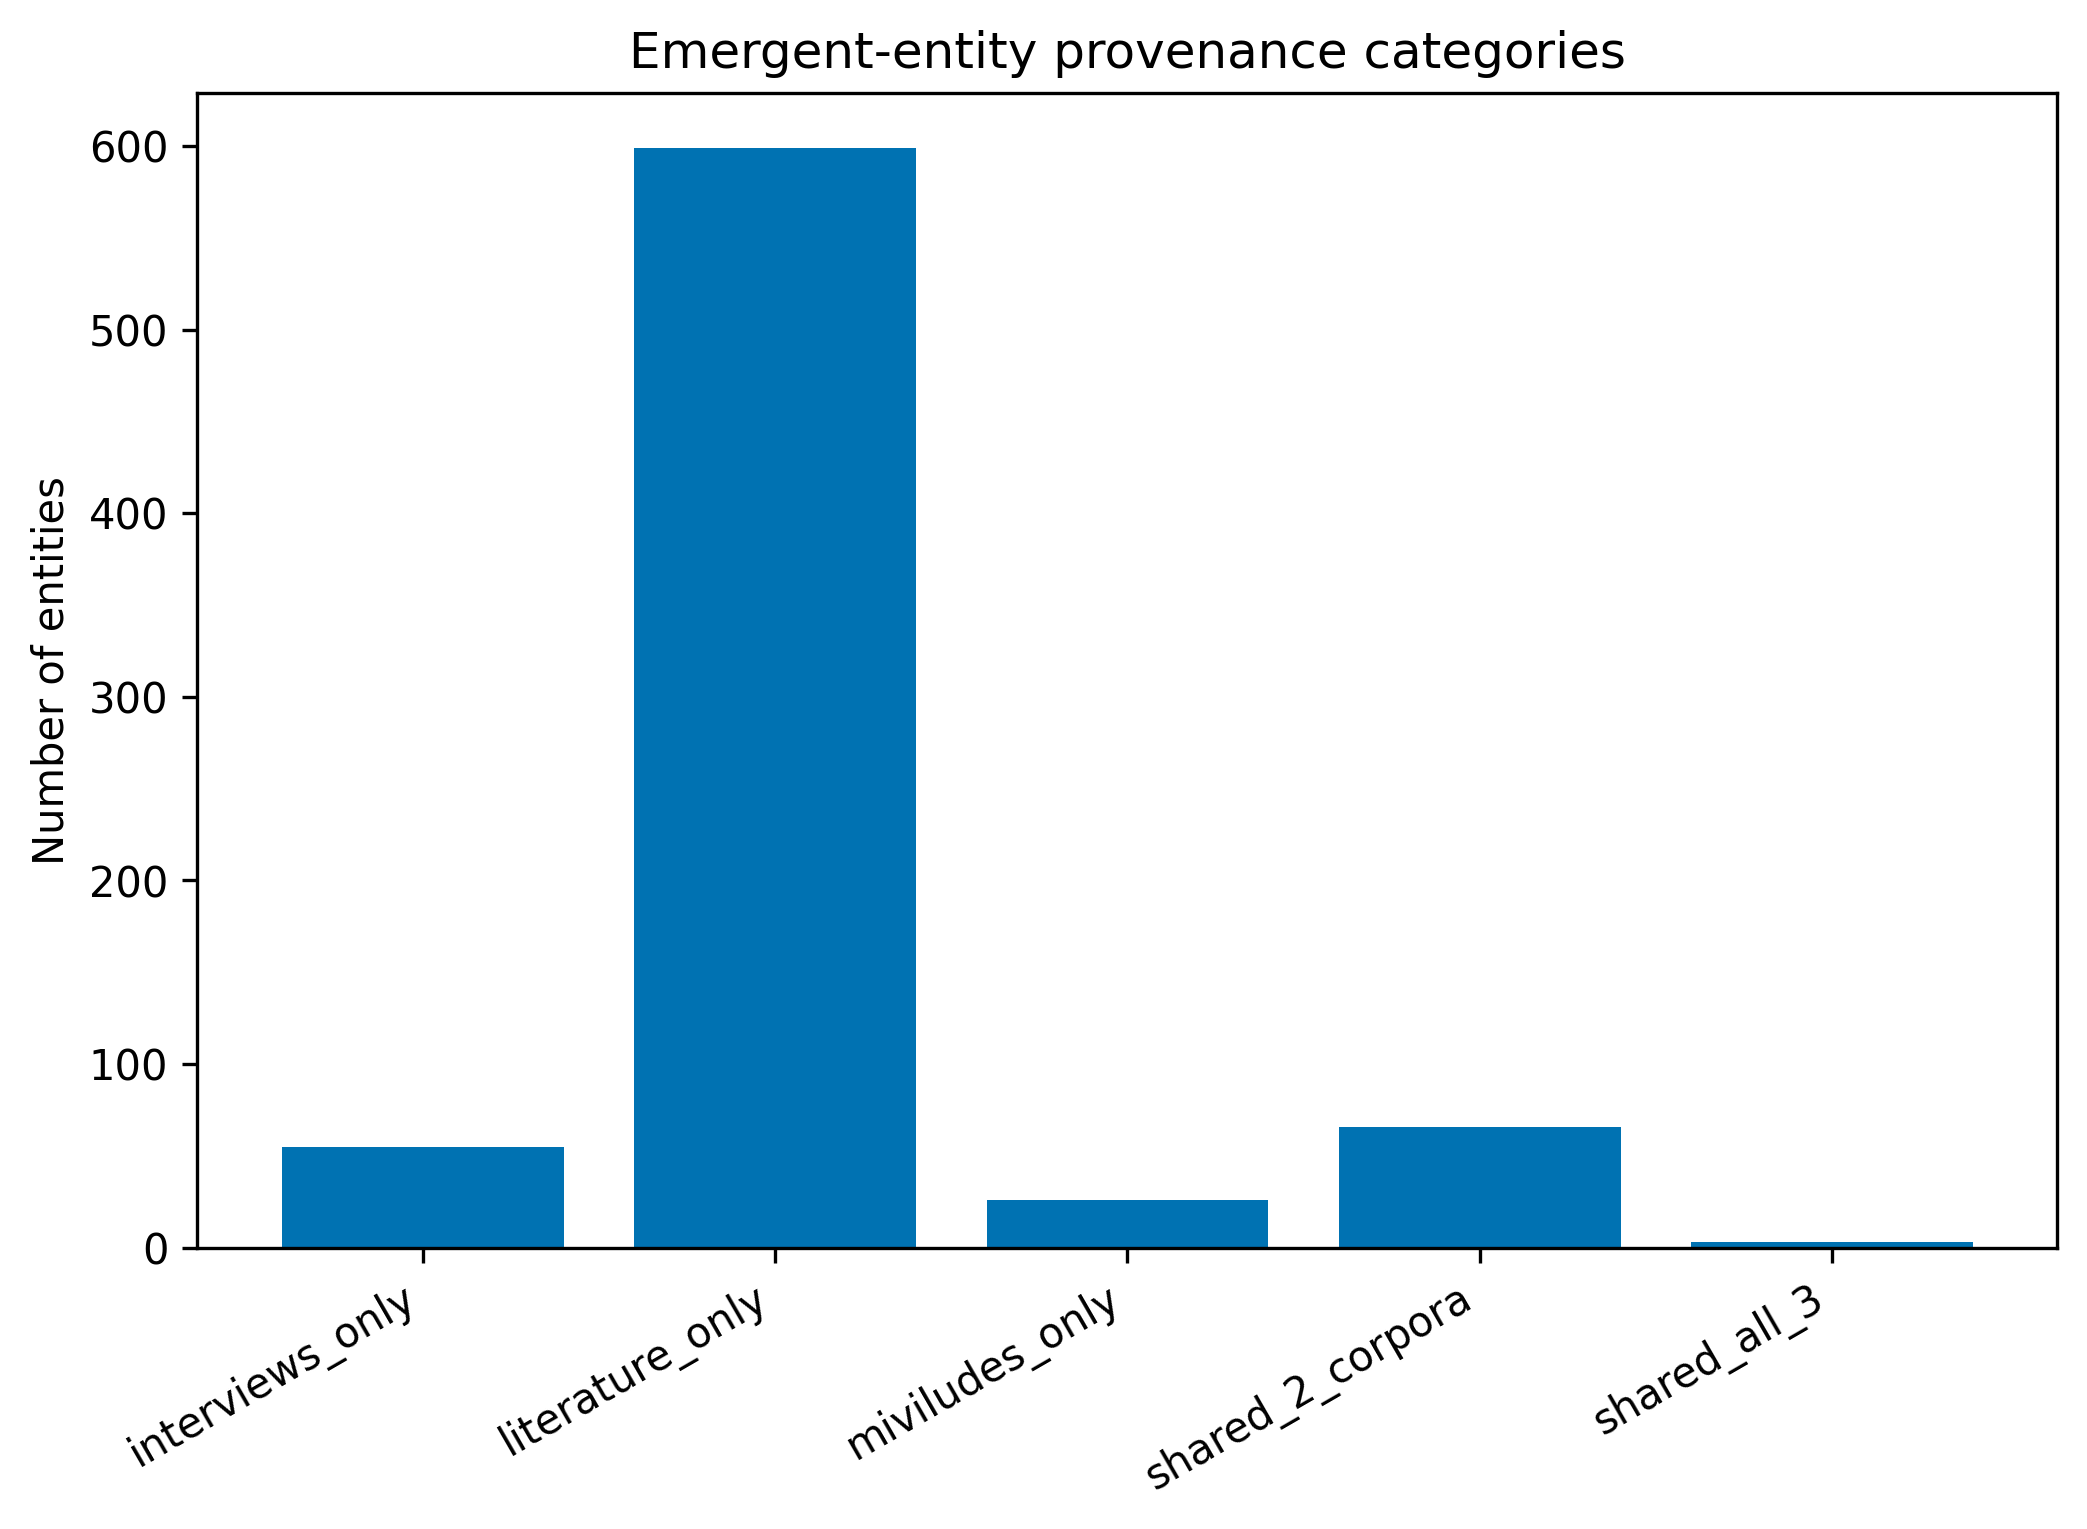
\includegraphics[width=0.7\textwidth]{figures/entity_provenance_categories.png}
\caption{Emergent entities grouped by which corpus/corpora mention them, this run.}
\end{figure}

Top entities by total mentions, unchanged in identity and rank from the
previous report (all 4 newly-excluded names sat in the long tail, not
the head): NRMs (685), Scientology (299), New Age (270), Heaven's Gate
(268), Unification Church (250), Jehovah's Witnesses (211), New
Religious Movements (195), Branch Davidians (159), Jonestown (156),
Solar Temple (136), Church of Scientology (133), Peoples Temple (129).

\textbf{The 3 entities mentioned by all three corpora}, unchanged: "new
age" (270 total: 259 literature, 9 miviludes, 2 interviews), "t\'emoins
de j\'ehovah" (9 total: 1/7/1), "ordre du temple solaire" (4 total:
2/1/1).

As before, this module does \textbf{not} classify any entity as
"genuinely a cult" versus "mainstream" or apply any other normative
label -- it reports who talks about what, not who is right.

% ============================================================
\section{Epistemic status of emergent entities: what's asserted, what's negated, what's unknown}
\label{sec:epistemic}
% ============================================================

This section directly answers a question raised about the previous
report: entities are pooled purely by \emph{mention}, with no regard to
whether the text asserted, denied, or merely speculated about them --
"X is a cult," "X is NOT a cult," and "X might be a cult" all
contributed identically to the same entity point. This section reports
what tracking that distinction, per entity, actually finds.

\begin{table}[h!]
\centering
\begin{tabular}{lr}
\toprule
Mention tag & Count, across all 16{,}828 entity mentions \\
\midrule
unknown (no stance available) & 16{,}823 \\
asserted & 4 \\
speculative & 1 \\
negated & 0 \\
contested & 0 \\
qualified & 0 \\
\bottomrule
\end{tabular}
\caption{Every emergent-entity mention's own epistemic-status tag,
summed across all 749 entities.}
\end{table}

\begin{table}[h!]
\centering
\begin{tabular}{lll}
\toprule
Entity & Total mentions & Known-status breakdown \\
\midrule
nrms & 685 & asserted: 3; unknown: 682 \\
shakers & 35 & asserted: 1; unknown: 34 \\
koresh & 22 & speculative: 1; unknown: 21 \\
\bottomrule
\end{tabular}
\caption{The \textbf{only 3 of 749} entities carrying any mention with a
known (non-"unknown") epistemic tag. Every other entity's mentions are
100\% "unknown."}
\end{table}

\textbf{Why the "unknown" bucket dominates so completely}: only mentions
sourced from \texttt{entity\_anchors} carry a real per-mention stance,
inherited from that mention's own parent expression -- and
\texttt{entity\_anchors} is the smaller, stricter of the two extraction
fields (Section~\ref{sec:entities}). The much larger
\texttt{domain\_terms} field, responsible for the bulk of total mentions
(16{,}823 of 16{,}828, 99.97\%), is extracted at chunk level with no
expression-level claim attached to any individual mention, so it has no
stance to report -- every \texttt{domain\_terms}-sourced mention is
tagged "unknown," never guessed as "asserted." This is a real, load-
bearing limit on what this breakdown can currently answer, not an
artefact of how the tally itself works: as long as most entity signal
comes through \texttt{domain\_terms}, most of it will read as
epistemically unknown by construction.

\begin{plainbox}[What this does and does not show]
This finds no negated, contested, or qualified mentions of \emph{any}
entity in the emergent-entities layer at all, and only 5 asserted/
speculative mentions total across 3 entities. That is \textbf{not}
evidence that this corpus never denies or hedges on a named group --
denial and hedging are visible at the \emph{expression} level throughout
this project (\texttt{epistemic\_status} is a standard field on every
expression point, used elsewhere in this toolkit) -- it is evidence that
those expression-level stances are not currently propagated down to the
\emph{entity} layer for the great majority of entity mentions, because
most entity signal does not come from a stance-carrying field in the
first place. A future extraction pass that tags \texttt{domain\_terms}
mentions with their own local stance (rather than only the survivor
\texttt{entity\_anchors} field) would be the direct way to close this
gap; not attempted this run.
\end{plainbox}

% ============================================================
\section{Cross-corpus gap analysis}
\label{sec:crossgaps}
% ============================================================

New this run, built directly on the researcher's own framing: given
three very differently-motivated corpora -- an academic literature
review, a French state agency's operational reports, and 25 lay
interviews -- which regions of one corpus's own "entity space" are
\emph{not} occupied by another, and the reverse, for every pair. Two
complementary checks, deliberately kept separate (they answer different
questions):

\begin{itemize}[leftmargin=1.4em]
  \item \textbf{Lightweight}: on the existing 49 unified entity clusters
  (Section~\ref{sec:topology}), which corpora have zero members at all
  in a given cluster -- an exact-string-overlap check.
  \item \textbf{Heavier}: cluster each corpus's own entities
  \emph{independently}, then measure the geometric distance from each
  resulting cluster to the nearest entity the \emph{other} corpus
  mentions at all -- catching coverage the lightweight check cannot,
  since it does not require the same normalized string on both sides.
\end{itemize}

\begin{plainbox}[Governing principle]
Both checks report purely geometric facts about this embedding space
under this model. No numeric "this counts as a real gap" distance
threshold is invented anywhere below -- raw distances are reported, and
judging which are large enough to matter is left to the researcher,
read alongside this space's other established distance scales (e.g.\
Section~\ref{sec:results}'s own centroid-distance figures) rather than
decided silently in code.
\end{plainbox}

\subsection{Lightweight check: exact-entity coverage per cluster}

Of the 49 unified entity clusters: \textbf{0} have zero literature
presence, \textbf{40} have zero MIVILUDES presence, \textbf{28} have
zero interviews presence -- literature's much larger volume means it
touches essentially every cluster, while MIVILUDES (108 expressions, 2
documents) and interviews (64 expressions, 25 people) each leave large
parts of the shared entity space untouched by their own vocabulary
alone.

\begin{table}[h!]
\centering
\small
\begin{tabular}{p{0.7cm}p{9.5cm}}
\toprule
Cluster & Example members (cluster absent from both MIVILUDES and interviews) \\
\midrule
0 & anton lavey; lavey; timothy mcveigh \\
1 & buxton; dixon; marlene dixon \\
4 & aum; aum shinriky\={o}; aum shinrikyo; shinto; tenrikyo \\
5 & sai baba; sathya sai baba; shirdi sai baba \\
\bottomrule
\end{tabular}
\caption{4 of the 26 clusters with zero MIVILUDES-and-zero-interviews
presence -- specific named groups/figures discussed at length in
literature that neither of the other two corpora mention by these exact
strings at all. Full 26-row table in
\texttt{analyze\_entity\_topology/cluster\_corpus\_coverage.csv}. Note
cluster 1 ("dixon," "buxton") is a likely instance of
Section~\ref{sec:entities}'s known residual: Marlene Dixon and colleagues
are externally-cited scholars in this literature, not the topic itself
-- flagged rather than treated as a genuine finding.}
\end{table}

\begin{table}[h!]
\centering
\small
\begin{tabular}{p{0.7cm}p{9.5cm}}
\toprule
Cluster & Example members (all three corpora present) \\
\midrule
6 & order of the solar temple; ordo templi orientis; ordre du temple solaire; solar temple \\
13 & la secte de ra\"el; le truc de ra\"el; rael; raelians; ra\"elism \\
15 & d\'erives sectaires; jugendsekten; les d\'erives sectaires; sects; sekte; une secte. \\
25 & hare krishna; hare krishna movement; hare krishnas; the hare krishnas \\
\bottomrule
\end{tabular}
\caption{4 of the 7 clusters with at least one member mentioned by all
three corpora -- specific, well-known groups (Solar Temple, Ra\"elism,
Hare Krishna) plus one purely generic-vocabulary cluster (sect/secte/
sekte itself). Full table in the same CSV as above.}
\end{table}

\subsection{Heavier check: independent per-corpus clustering, geometric proximity}

Each corpus's own entities (those it mentions at all) were clustered
independently: literature (667 entities) into \textbf{47} clusters
(457 noise), MIVILUDES (47 entities) into \textbf{2} clusters (12
noise), interviews (107 entities) into \textbf{8} clusters (70 noise).
MIVILUDES's own institutional vocabulary is dominated by one large,
heterogeneous 32-member cluster (regulatory/administrative terms mixed
with a handful of named groups: "dgccrf," "cnrs," "miviludes,"
"l.\ ron hubbard," "the church universal and triumphant," "steiner-
waldorf") plus one small, purely generic 3-member cluster ("d\'erives
sectaires," "les d\'erives sectaires," "strat\'egie nationale de lutte
contre les d\'erives sectaires").

\begin{table}[h!]
\centering
\small
\begin{tabular}{p{2.6cm}p{4.2cm}p{2.3cm}p{1.5cm}}
\toprule
Corpus-A cluster & Corpus-A members (excerpt) & Nearest corpus-B entity & Distance \\
\midrule
\multicolumn{4}{l}{\textit{Closest lexically-different matches (literature $\to$ interviews)}} \\
lit.\ cl.\ 16 & moonie; moonies; the moonies & interviews: moonies & 7.06 \\
lit.\ cl.\ 42 & church of scientology; scientology & interviews: church of scientology & 7.71 \\
lit.\ cl.\ 43 & mormon; mormon church; mormonism & interviews: mormons & 8.64 \\
\multicolumn{4}{l}{\textit{Farthest matches (literature $\to$ MIVILUDES) -- candidate gaps}} \\
lit.\ cl.\ 7 & charles manson; manson; manson family & miviludes: l.\ ron hubbard & 38.89 \\
lit.\ cl.\ 2 & clapham; clapham sect; the clapham sect & miviludes: les d\'erives sectaires & 39.39 \\
lit.\ cl.\ 9 & people's temple; peoples temple & miviludes: ordre du temple solaire & 40.00 \\
lit.\ cl.\ 16 & moonie; moonies; the moonies & miviludes: toujours renouvel\'ees & 40.56 \\
\bottomrule
\end{tabular}
\caption{Selected rows from \texttt{cross\_corpus\_cluster\_proximity.csv}
(114 rank-1 rows total, 6 directional corpus pairs). Read together: the
same literature clusters that sit very close to an interview entity
(Moonies $\to$ "moonies," 7.06) sit among the \emph{farthest} from any
MIVILUDES entity (Moonies $\to$ "toujours renouvel\'ees," 40.56) --
MIVILUDES's institutional-report vocabulary and lay interviewees'
pop-culture-inflected vocabulary independently converge on some of the
same well-known named groups literature discusses, while MIVILUDES's own
vocabulary does not name several of literature's most historically
notorious groups (Manson Family, Peoples Temple, Clapham Sect) at all.}
\end{table}

Read across all 6 directional pairs (full table, 114 rank-1 rows, in the
CSV): the closest cross-corpus matches found were overwhelmingly the
\emph{same} entity under near-identical wording (e.g.\ "scientology"
$\leftrightarrow$ "church of scientology"), not a genuinely different
lexical form for the same referent (the module's own worked example --
"Peoples Temple" vs.\ "Jonestown" -- did not itself appear among the
closest-match rows this run, though both terms exist as separate
literature clusters); reported honestly rather than claimed as
demonstrated, since the mechanism that would catch a case like that
(true synonym-level proximity rather than near-identical strings) was
not distinctly observed in this run's closest matches.

\begin{plainbox}[What this does and does not show]
A large distance from a corpus-A cluster to corpus-B's nearest entity is
consistent with a genuine coverage gap, but is equally consistent with:
(1) corpus B simply having very few entities overall to be near
anything (MIVILUDES: 47; interviews: 107), mechanically inflating
typical nearest-neighbour distances regardless of topical overlap; or
(2) the residual cited-author contamination noted in
Section~\ref{sec:entities} producing an artefactual cluster on the
corpus-A side. Neither check in this section classifies a gap as
meaningful on its own -- that judgment, and any decision about which
gaps are worth discussing in the Results chapter, is left to the
researcher.
\end{plainbox}

% ============================================================
\section{Per-interview extraction sanity-check aid}
\label{sec:qa-trace}
% ============================================================

New this run, directly answering the request for a way to manually
confirm, interview by interview, that extraction "makes sense" before
trusting the pooled numbers above. \texttt{qa\_interview\_entity\_trace.py}
reads the raw interview archive directly (not the shared space) and, for
each of the 25 interviews, lists every kept expression and every
\texttt{domain\_terms} mention from that interview, resolved forward
through the same filters Section~\ref{sec:entities} describes (named-
entity shape, embedded-at-all, cited-author stop-list, per-corpus
mention threshold) to whichever final pooled entity it became -- or the
exact filter it failed, if it did not survive.

Run against this session's data: \textbf{25} interviews, \textbf{64}
expressions, \textbf{331} \texttt{domain\_terms} mentions traced, of
which \textbf{127} (38\%) resolved to a pooled entity and \textbf{204}
(62\%) were filtered out for not being named-entity-shaped in the first
place (generic vocabulary like "cult," "hierarchy," "key members" --
already excluded by design, not a data-quality problem). No mentions in
this run were filtered for the other three reasons (not embedded, cited-
author surname, below mention threshold) -- expected for the cited-
author case, since interview participants are not citing this corpus's
own academic bibliography.

\begin{plainbox}[Not included in this document]
The trace's own CSV/PDF output (\texttt{processed/qa/interview\_entity\_
trace/}) embeds every kept expression's verbatim text at bulk scale --
appropriate for a local, researcher-facing sanity check, not for a
document meant to circulate as a thesis appendix, so it is gitignored
and regenerated locally via the script above rather than reproduced
here. This is a stricter standard than the modest number of individual
illustrative quotes already used elsewhere in this document (e.g.\
Section~\ref{sec:results}'s typicality examples) -- the difference is
scale (every kept expression from every interview, vs.\ a small,
deliberately chosen set of examples), not a claim that interview
excerpts can never appear in this report at all.
\end{plainbox}

% ============================================================
\section{Entity topology: clusters, density, gaps, centrality}
\label{sec:topology}
% ============================================================

Same three questions about the emergent entities as the previous
report, refreshed against the corrected 749-entity space, all answered
in the REAL 393-dimensional space (never a 2-D projection -- pictures
come after, as a reading aid).

\begin{plainbox}[Governing principle]
Cluster membership, local density, and centrality are purely geometric
facts about this embedding space under this model. A "dense cluster" of
entities is not itself evidence those entities are conceptually similar
in any deeper sense than "their extracted-context embeddings landed near
each other"; an HDBSCAN "noise" label does not mean an entity is
unimportant, only that it did not sit inside a density-defined cluster
at the chosen threshold.
\end{plainbox}

\texttt{sklearn.cluster.HDBSCAN} finds \textbf{49 clusters} among the
749 entities, at a minimum cluster size of 3; \textbf{512 entities
(68\%)} are noise at this threshold -- unchanged in proportion from the
previous report's 514/753.

\begin{table}[h!]
\centering
\small
\begin{tabular}{p{0.9cm}p{0.6cm}p{2.1cm}p{9.5cm}}
\toprule
Cluster & Size & Dist.\ to grand centroid & Members \\
\midrule
\multicolumn{4}{l}{\textit{Most central}} \\
15 & 6 & 20.53 & d\'erives sectaires; jugendsekten; les d\'erives sectaires; sects; sekte; une secte. \\
32 & 14 & 20.92 & center for studies on new religions; new age; new age movement; new religious movement(s); \ldots \\
23 & 10 & 21.90 & church of satan; satan; satanic; satanism; satanist(s); the cult of satan; \ldots \\
\multicolumn{4}{l}{\textit{Most peripheral}} \\
46 & 6 & 31.56 & catholic; catholic church; catholicism; catholics; roman catholic (church) \\
9 & 3 & 31.65 & clapham; clapham sect; the clapham sect \\
20 & 3 & 32.23 & moonie; moonies; the moonies \\
36 & 3 & 33.27 & california; los angeles; san francisco \\
35 & 4 & 33.32 & jehovah's witnesses; les t\'emoins de j\'ehovah; t\'emoins de j\'ehovah; zeugen jehovas \\
\bottomrule
\end{tabular}
\caption{Most central and most peripheral entity clusters, this run --
same clusters, same ranking as the previous report (cluster IDs shifted
slightly because HDBSCAN re-ran on 4 fewer entities). Full 49-cluster
table in \texttt{analyze\_entity\_topology/cluster\_summary.csv}.}
\end{table}

\begin{figure}[h!]
\centering
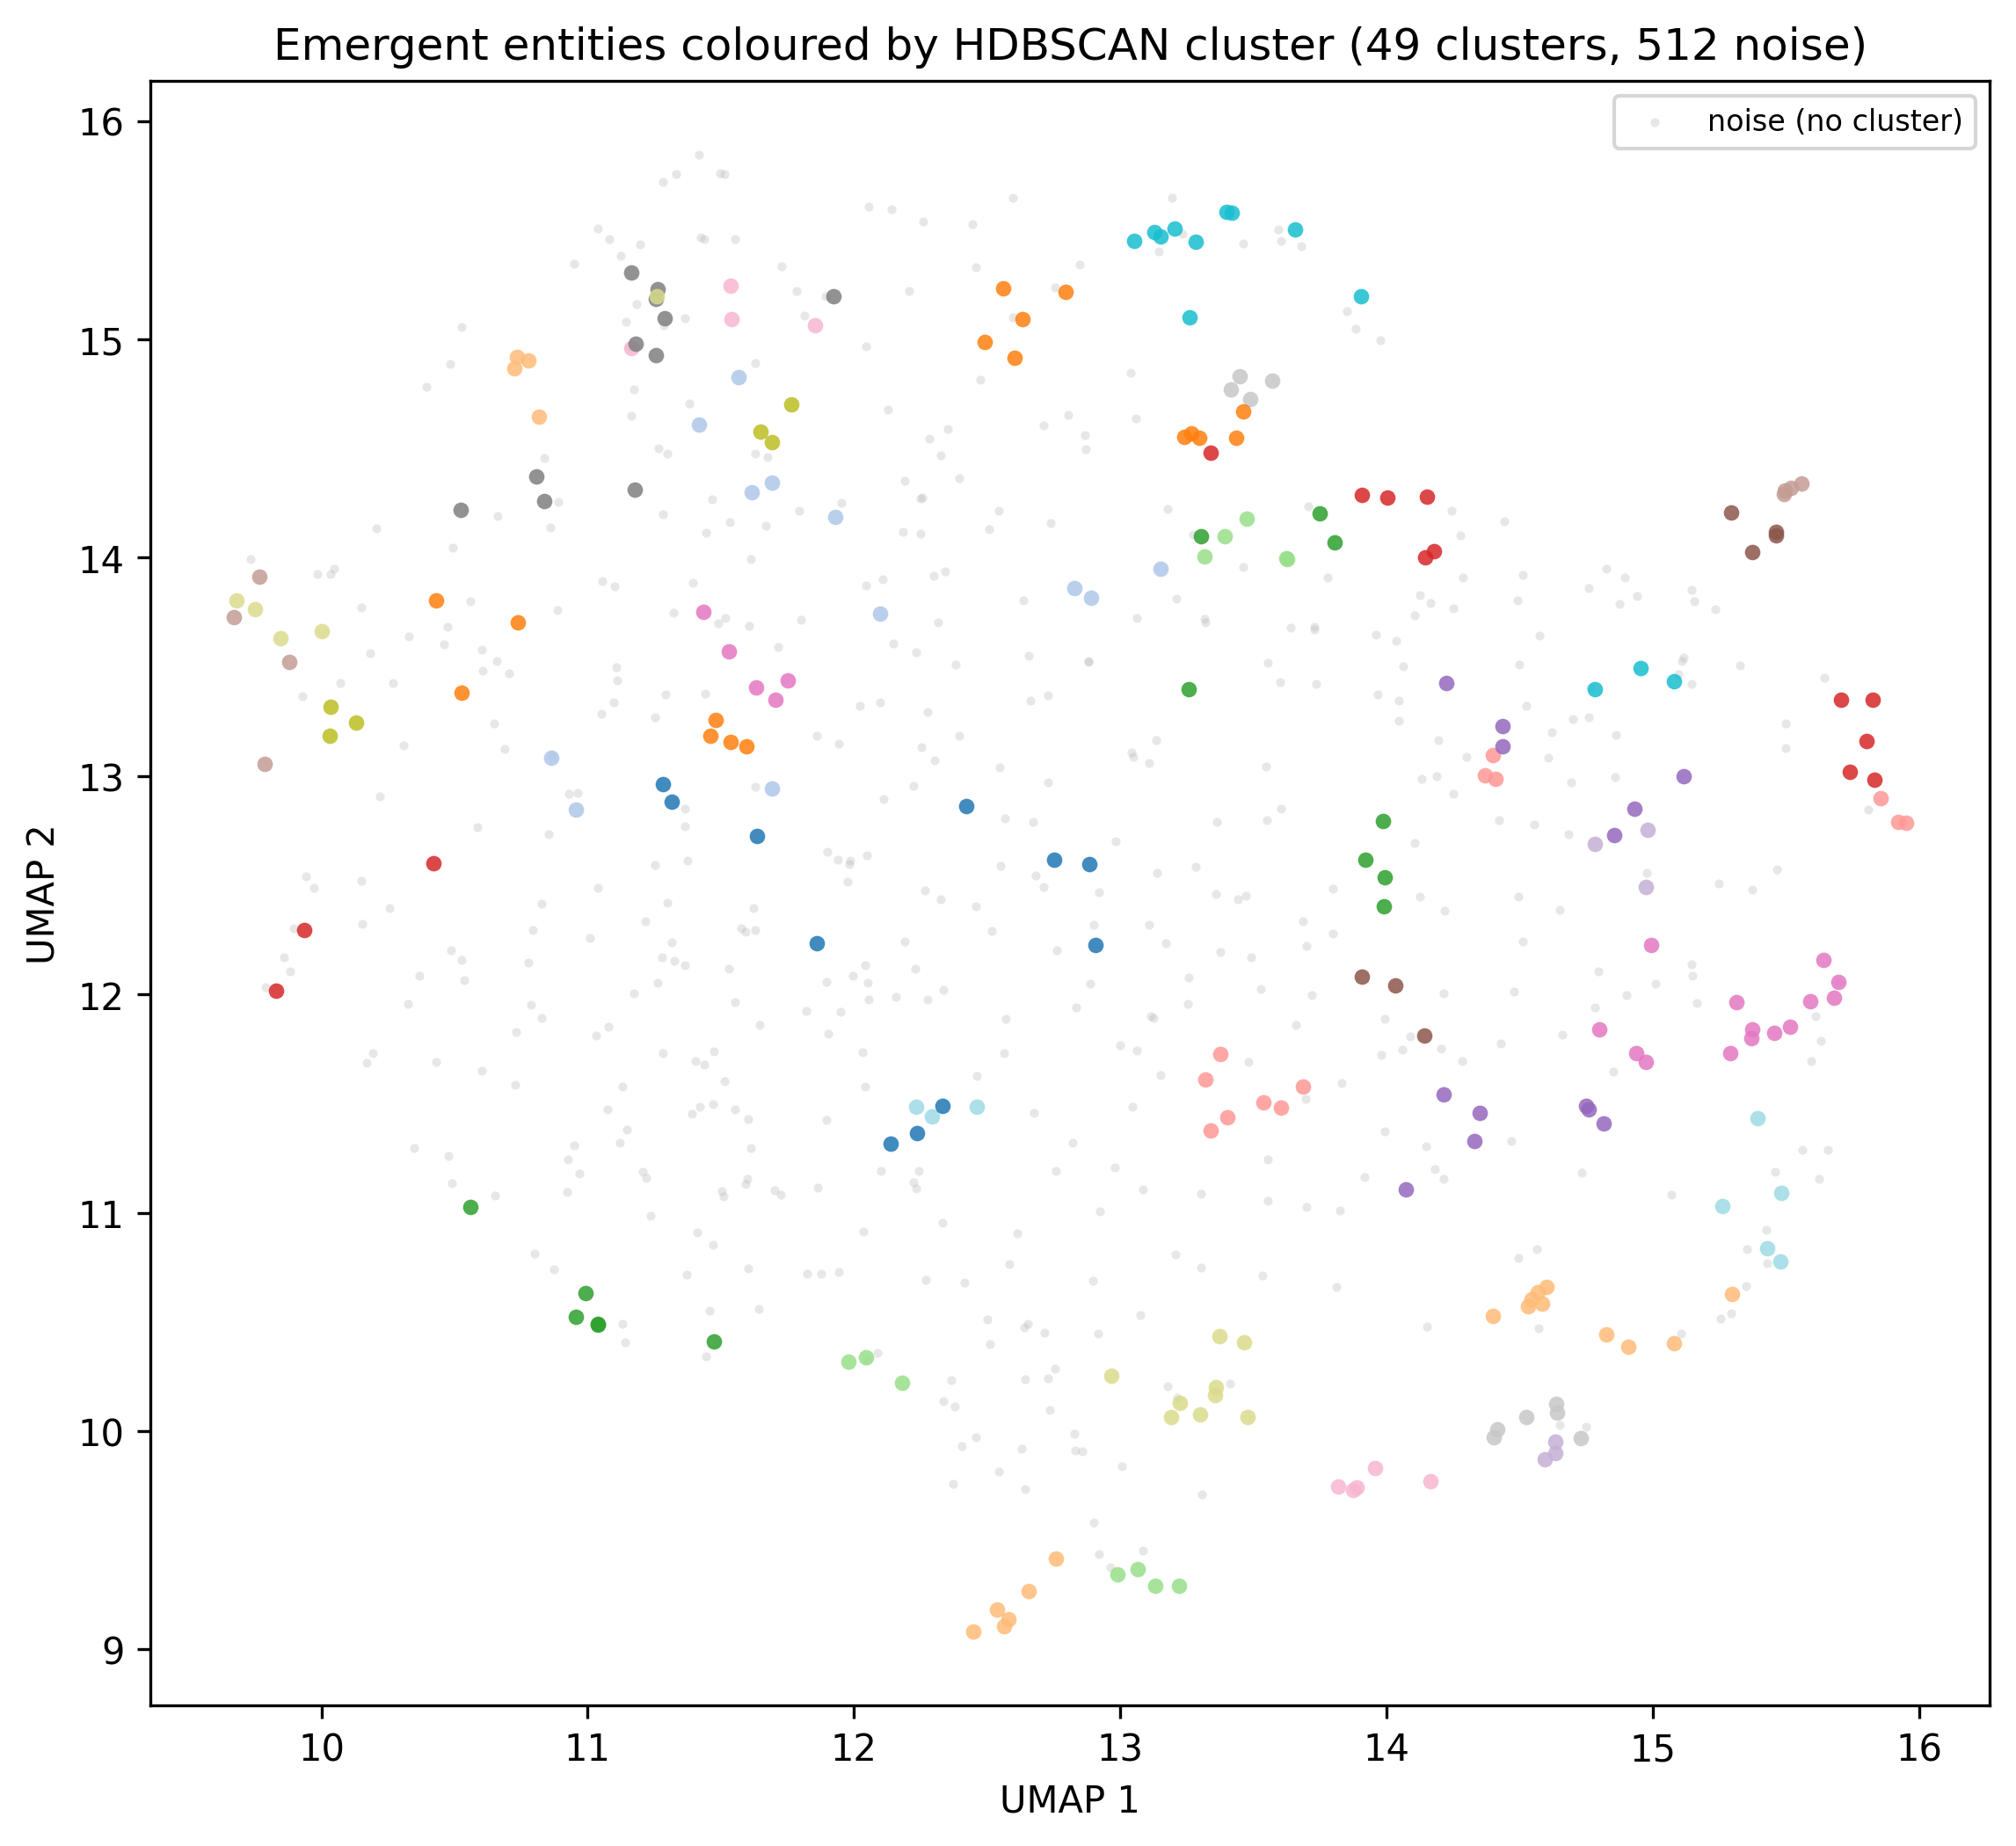
\includegraphics[width=0.85\textwidth]{figures/entity_clusters_umap.png}
\caption{The 749 entities, 2-D UMAP projection, coloured by HDBSCAN
cluster (grey = noise), this run.}
\end{figure}

\textbf{Coverage gaps} (same 2-D-grid method as before): \textbf{8 of
167} in-hull grid cells have zero entities -- down from 9/167, a change
of this scale fully consistent with removing 4 entities from a 749-point
layout.

\begin{figure}[h!]
\centering
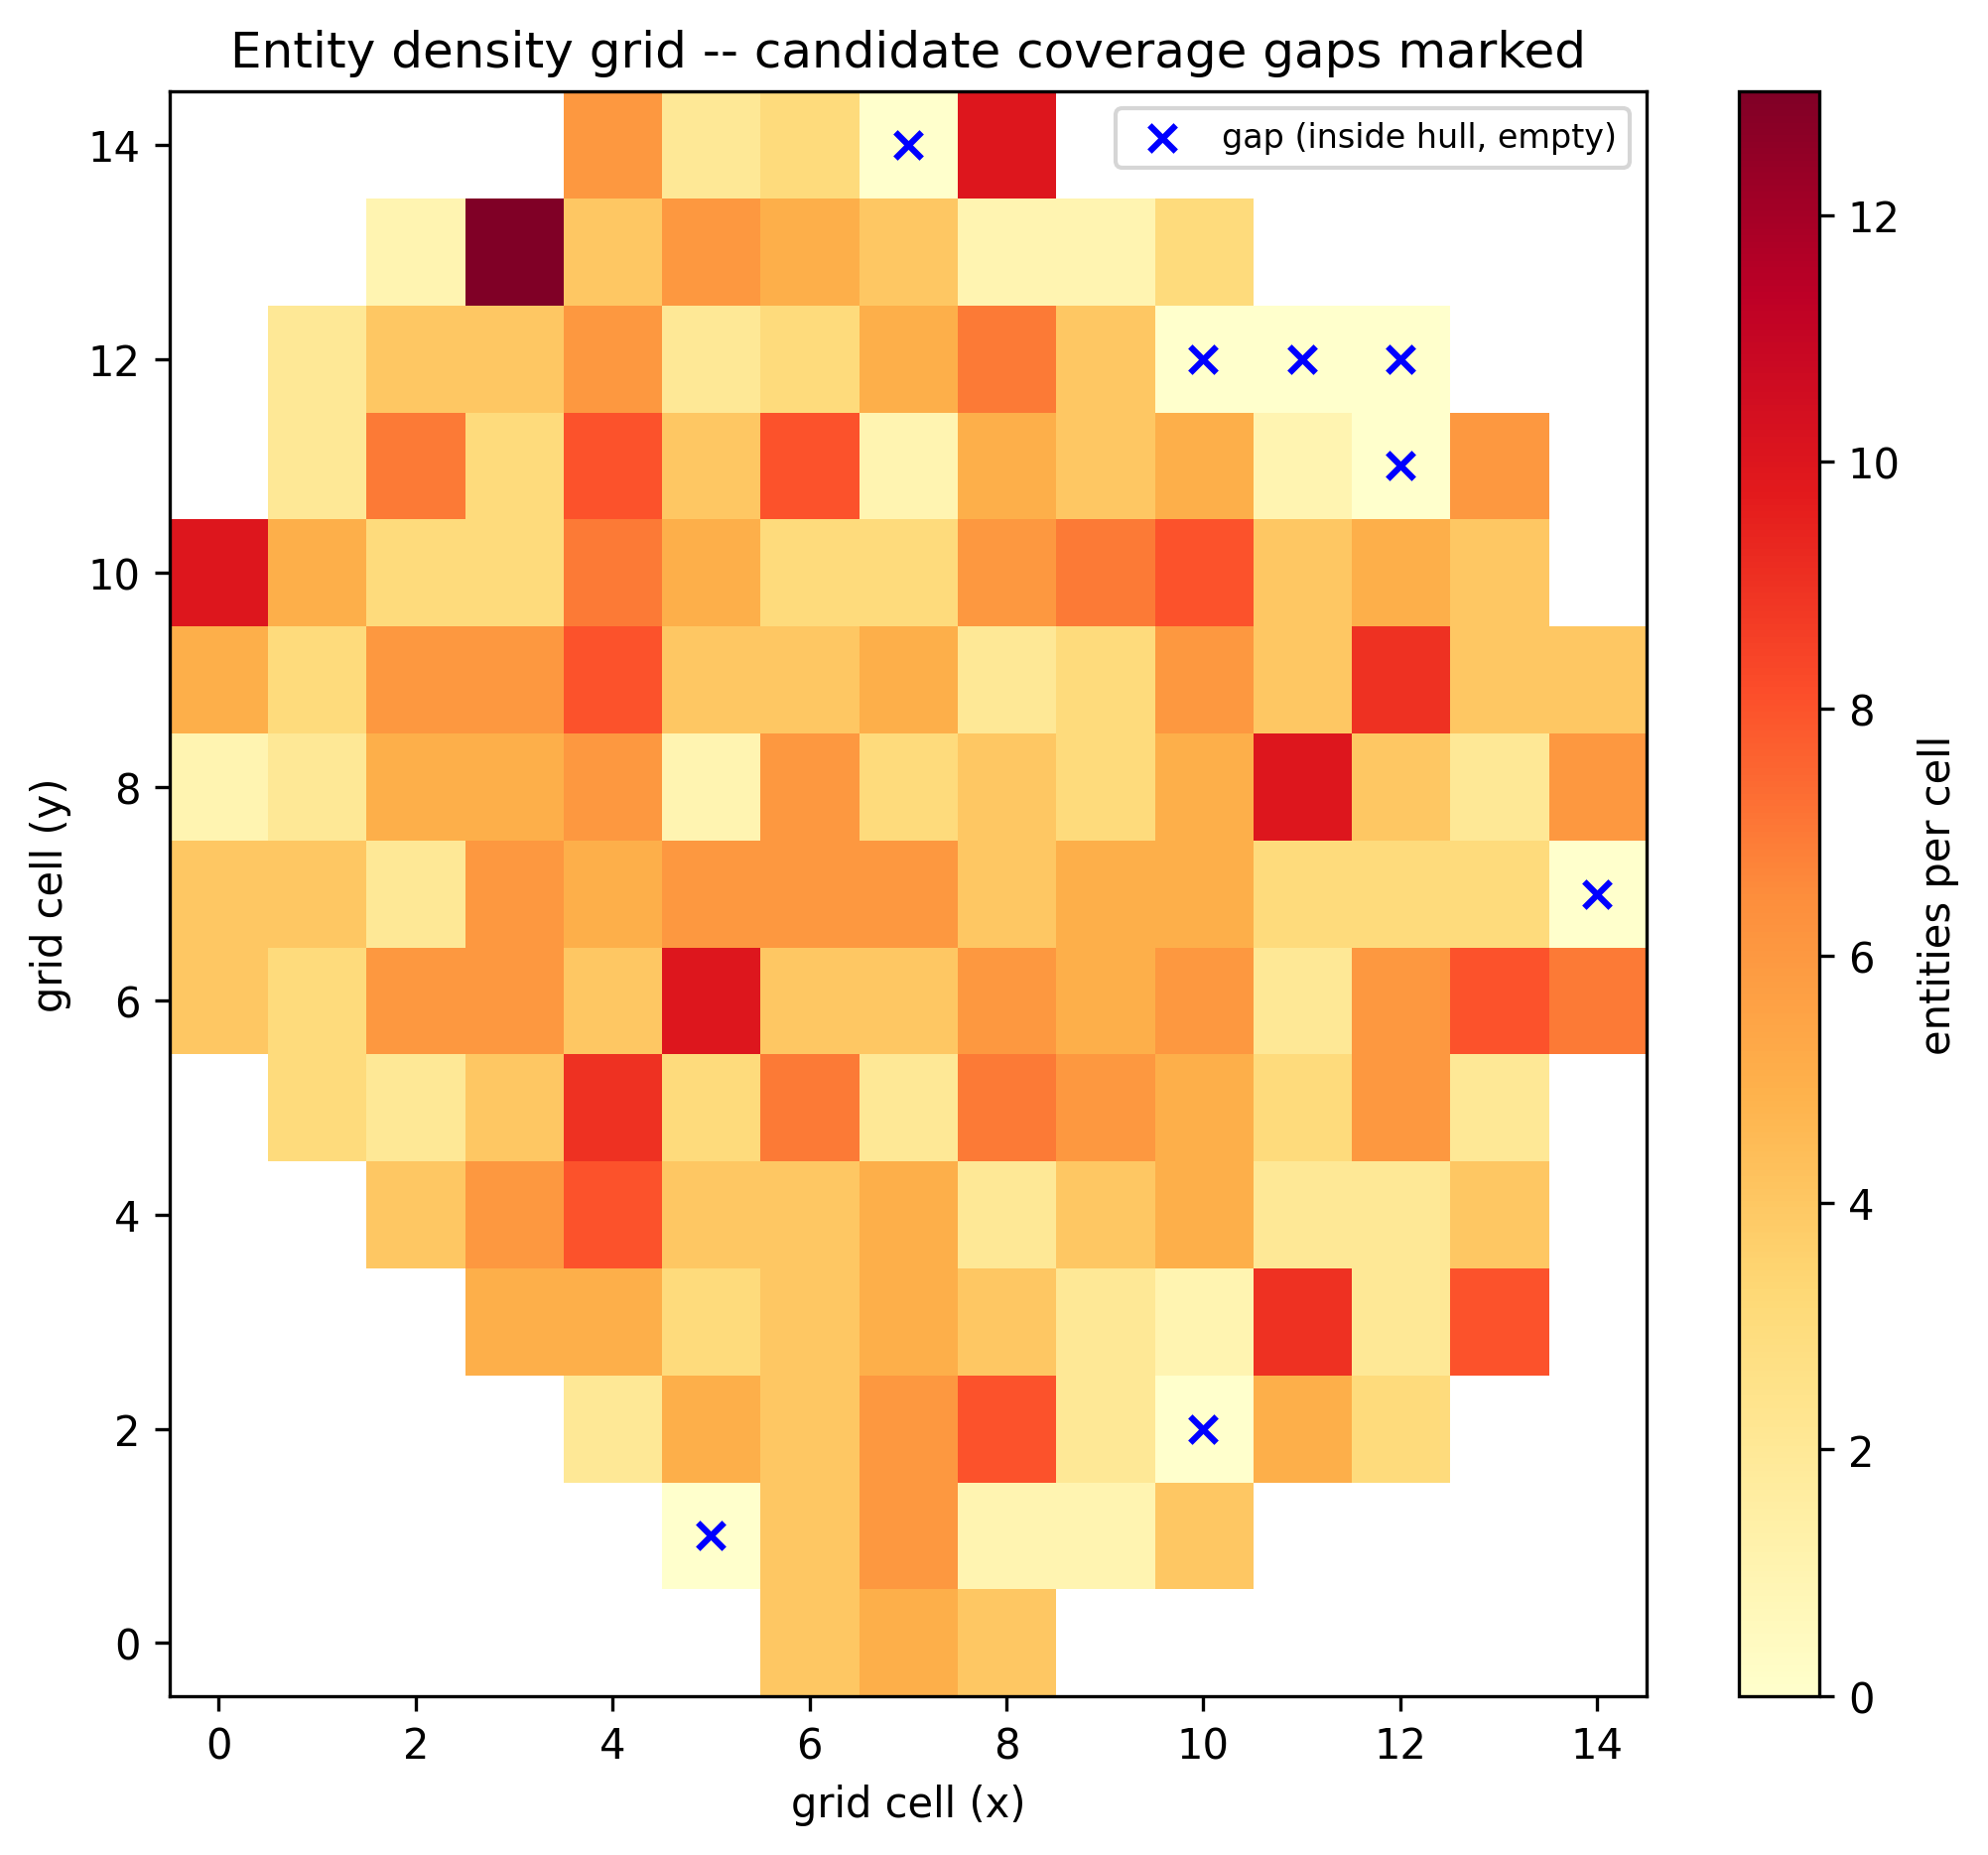
\includegraphics[width=0.8\textwidth]{figures/entity_gap_heatmap.png}
\caption{Entity count per grid cell (2-D UMAP layout), this run; blue
$\times$ marks a candidate gap.}
\end{figure}

% ============================================================
\section{Voronoi regions: three seed strategies, tried and compared}
\label{sec:voronoi}
% ============================================================

Unchanged conclusion from the previous report, refreshed against the
749-entity space: only the \textbf{cluster-centroid-seeded} strategy
(49 seeds, this run) produces a legible 2-D tessellation
(Figure~\ref{fig:voronoi-cluster}); the criteria-seeded (17 seeds) and
corpus-centroid-seeded (3 seeds) strategies both collapse into one
corner of the layout under UMAP's out-of-sample transform
(Figures~\ref{fig:voronoi-criteria}--\ref{fig:voronoi-corpus}), a
well-documented UMAP limitation, not evidence the criteria or corpora
are geometrically confused with each other. All high-dimensional
retrieval elsewhere in this document is computed directly in the real
393-D space and is unaffected by this 2-D projection artefact.

\begin{figure}[h!]
\centering
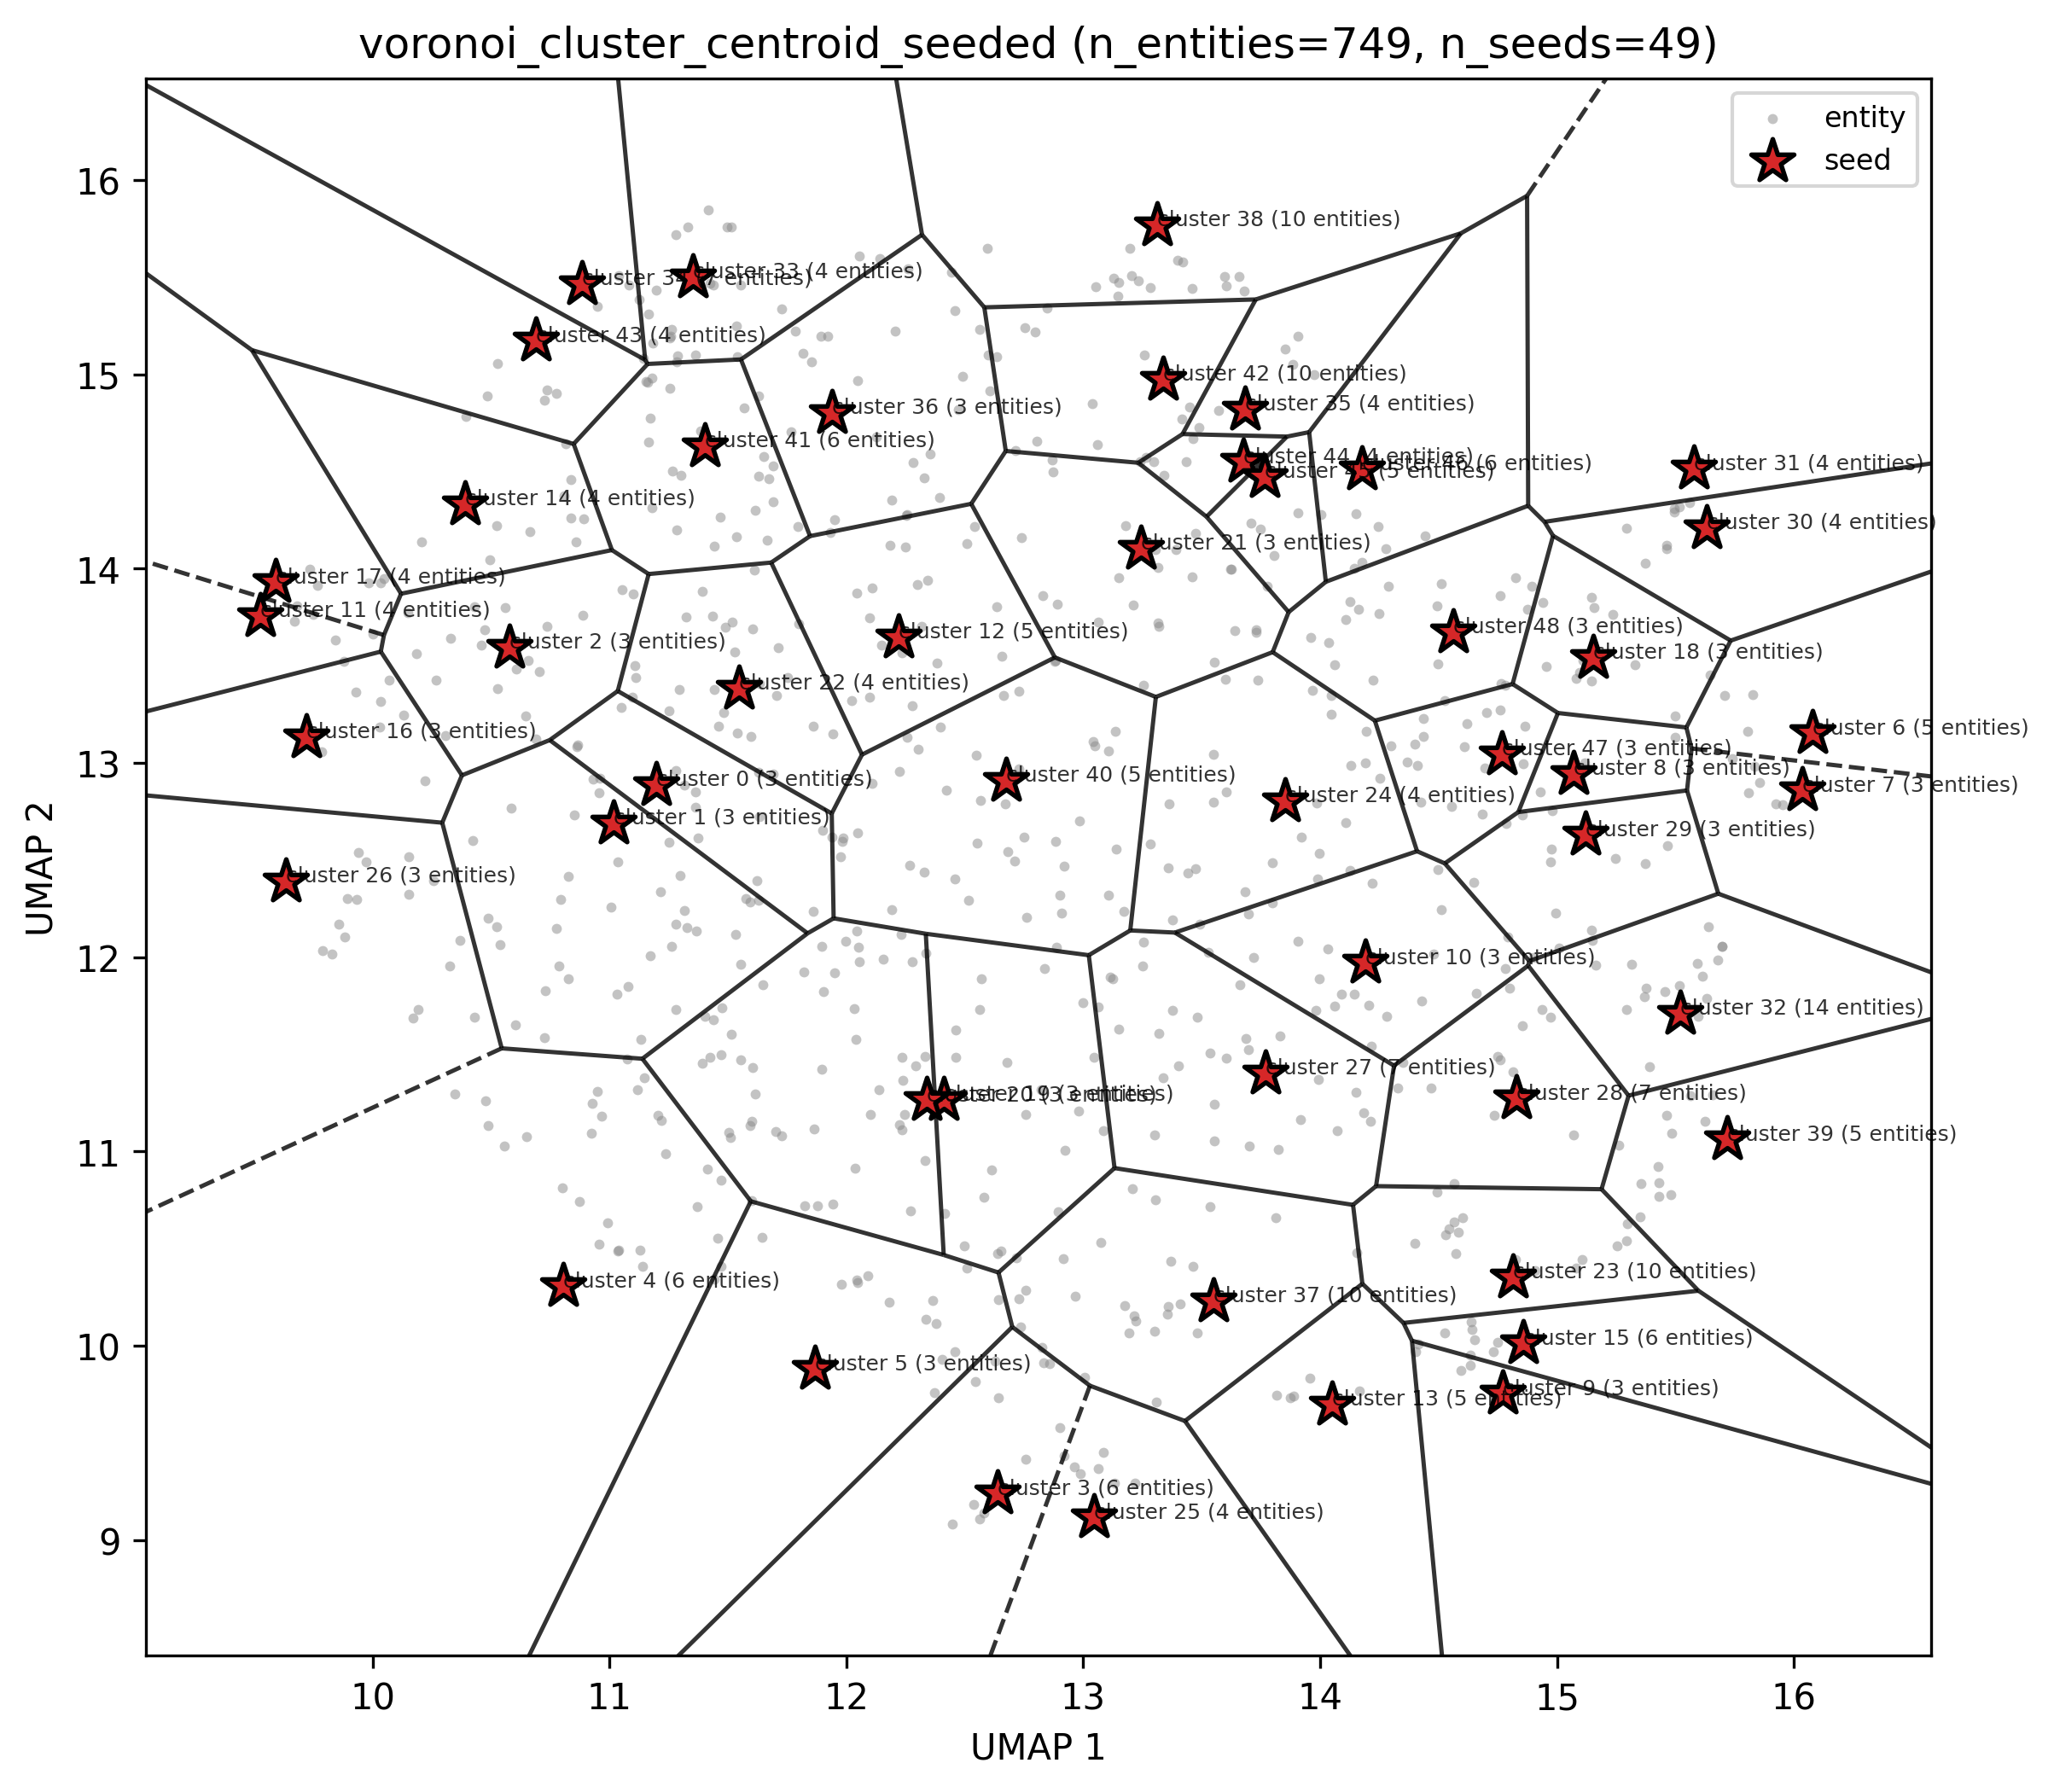
\includegraphics[width=0.85\textwidth]{figures/voronoi_cluster_centroid_seeded.png}
\caption{Cluster-centroid-seeded Voronoi tessellation, this run.}
\label{fig:voronoi-cluster}
\end{figure}

\begin{figure}[h!]
\centering
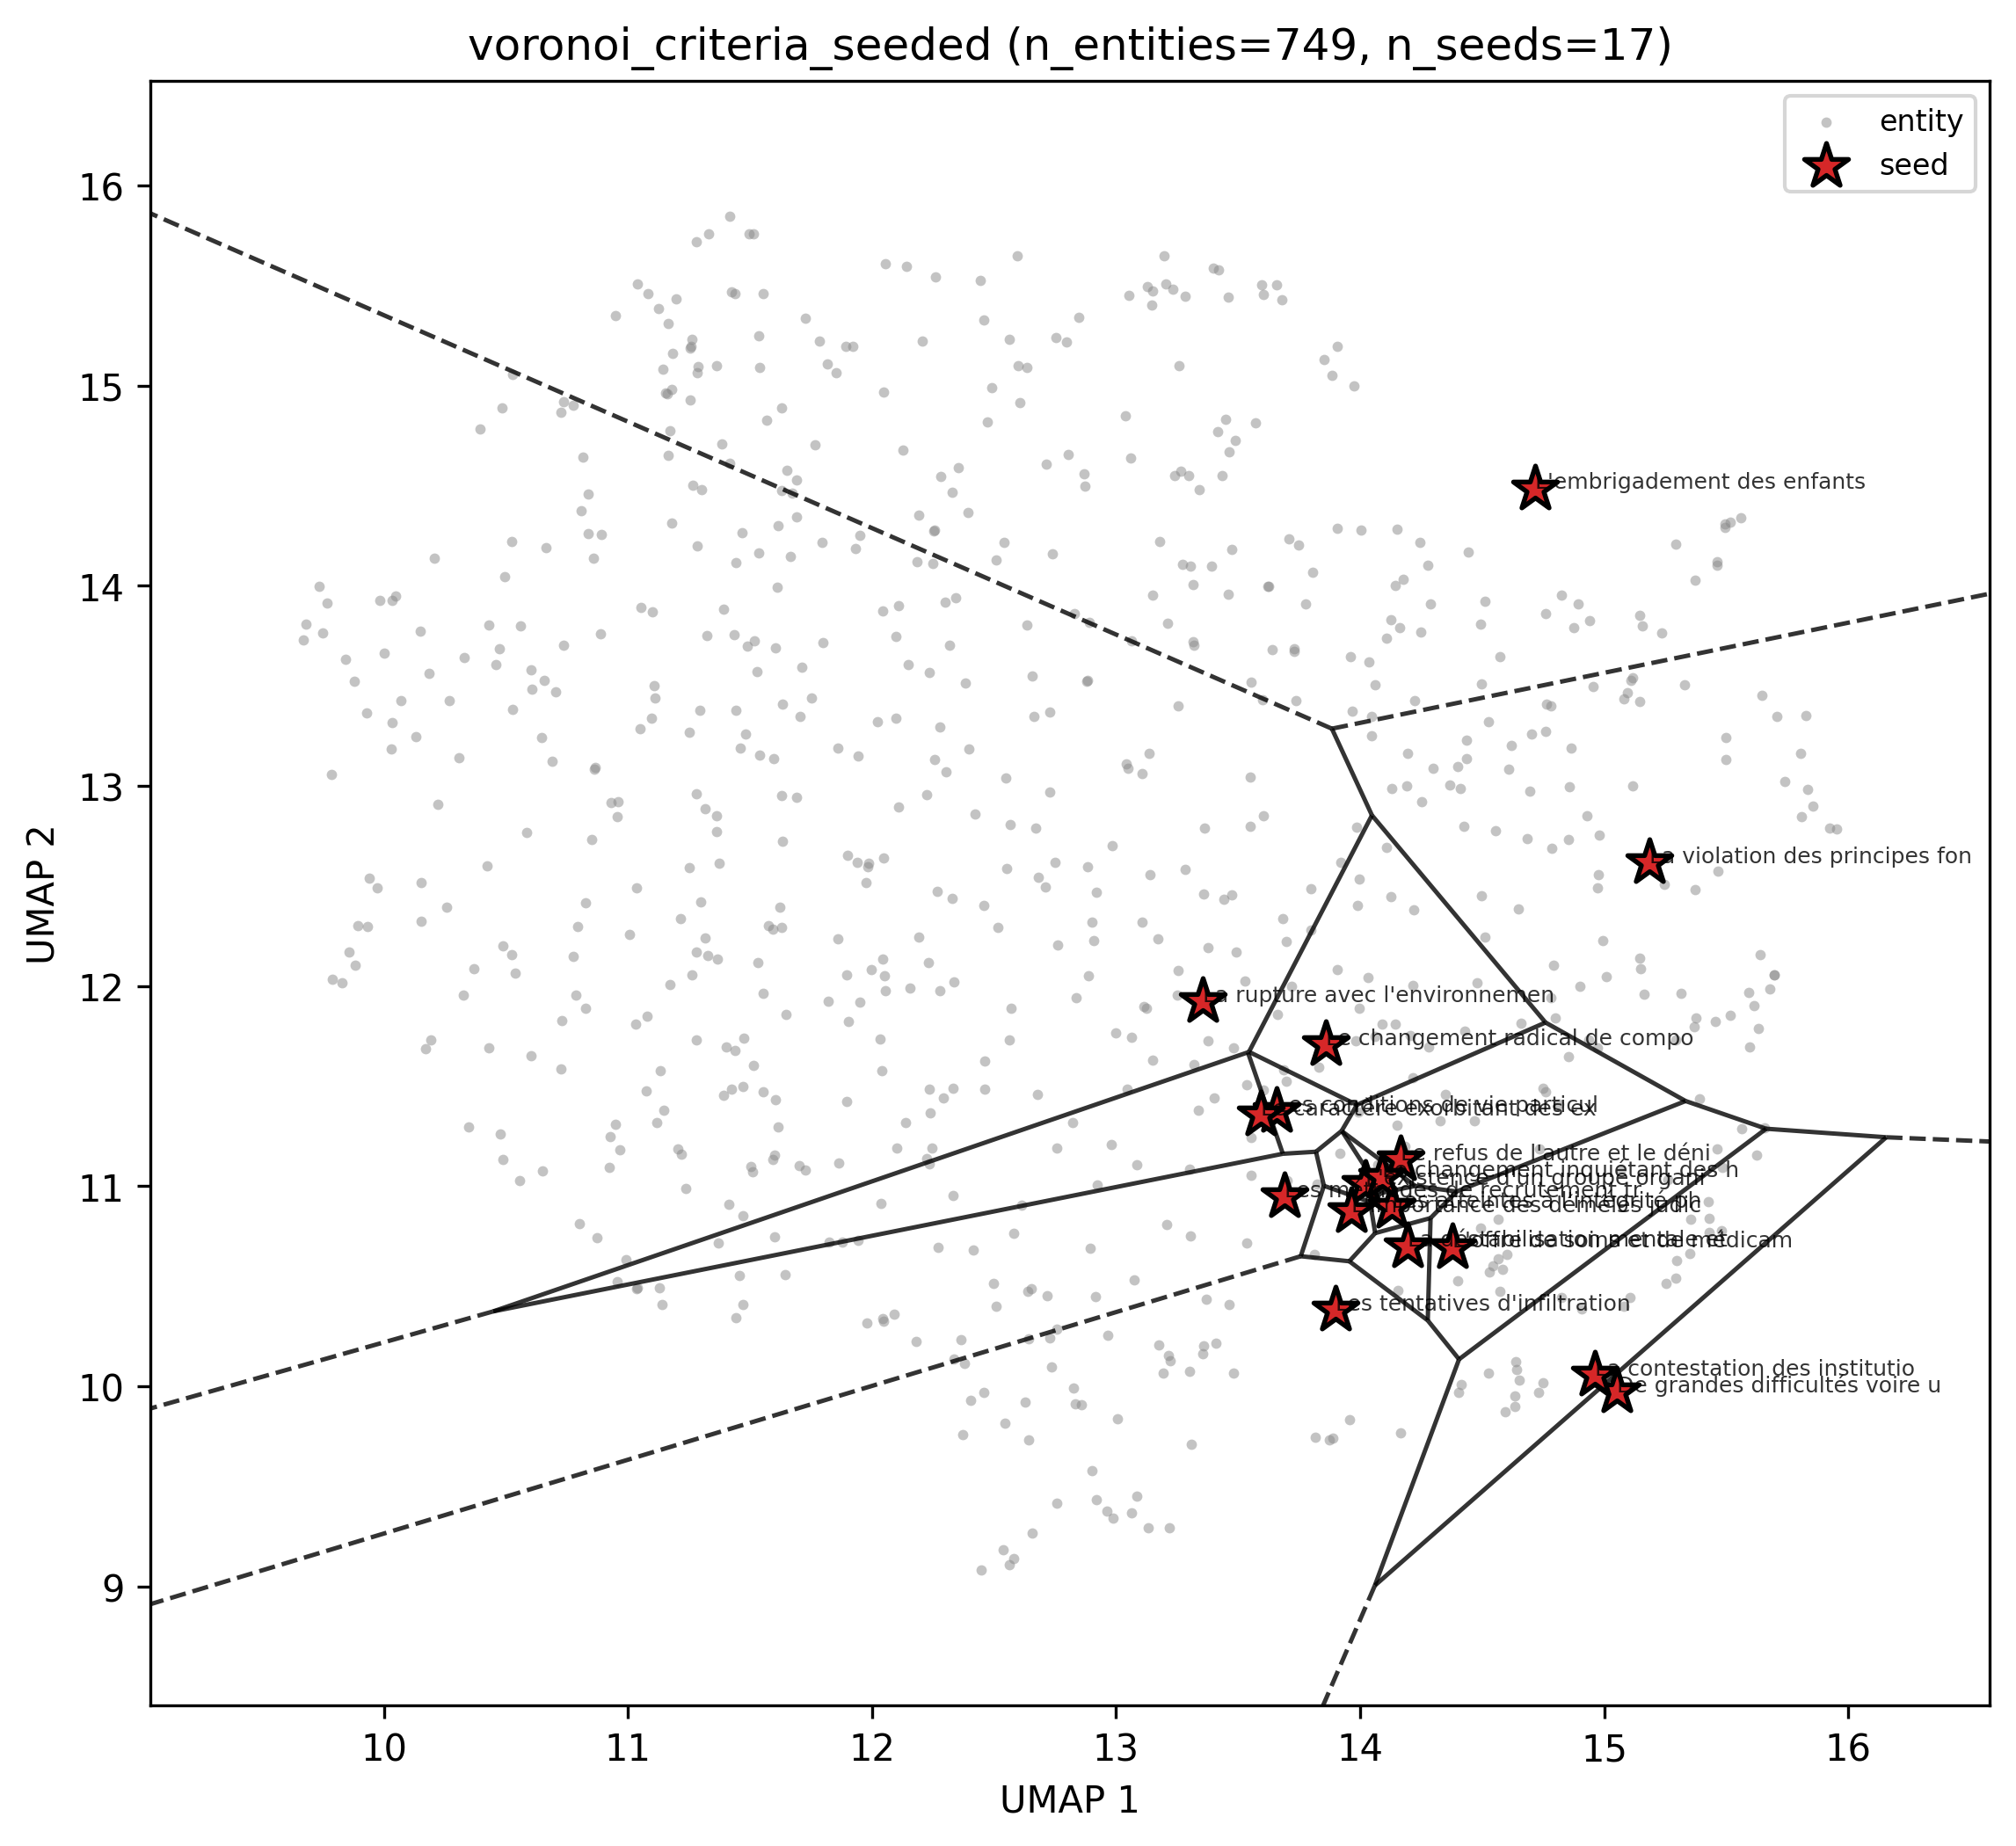
\includegraphics[width=0.75\textwidth]{figures/voronoi_criteria_seeded.png}
\caption{Criteria-seeded attempt -- included for honesty about what was
tried, this run.}
\label{fig:voronoi-criteria}
\end{figure}

\begin{figure}[h!]
\centering
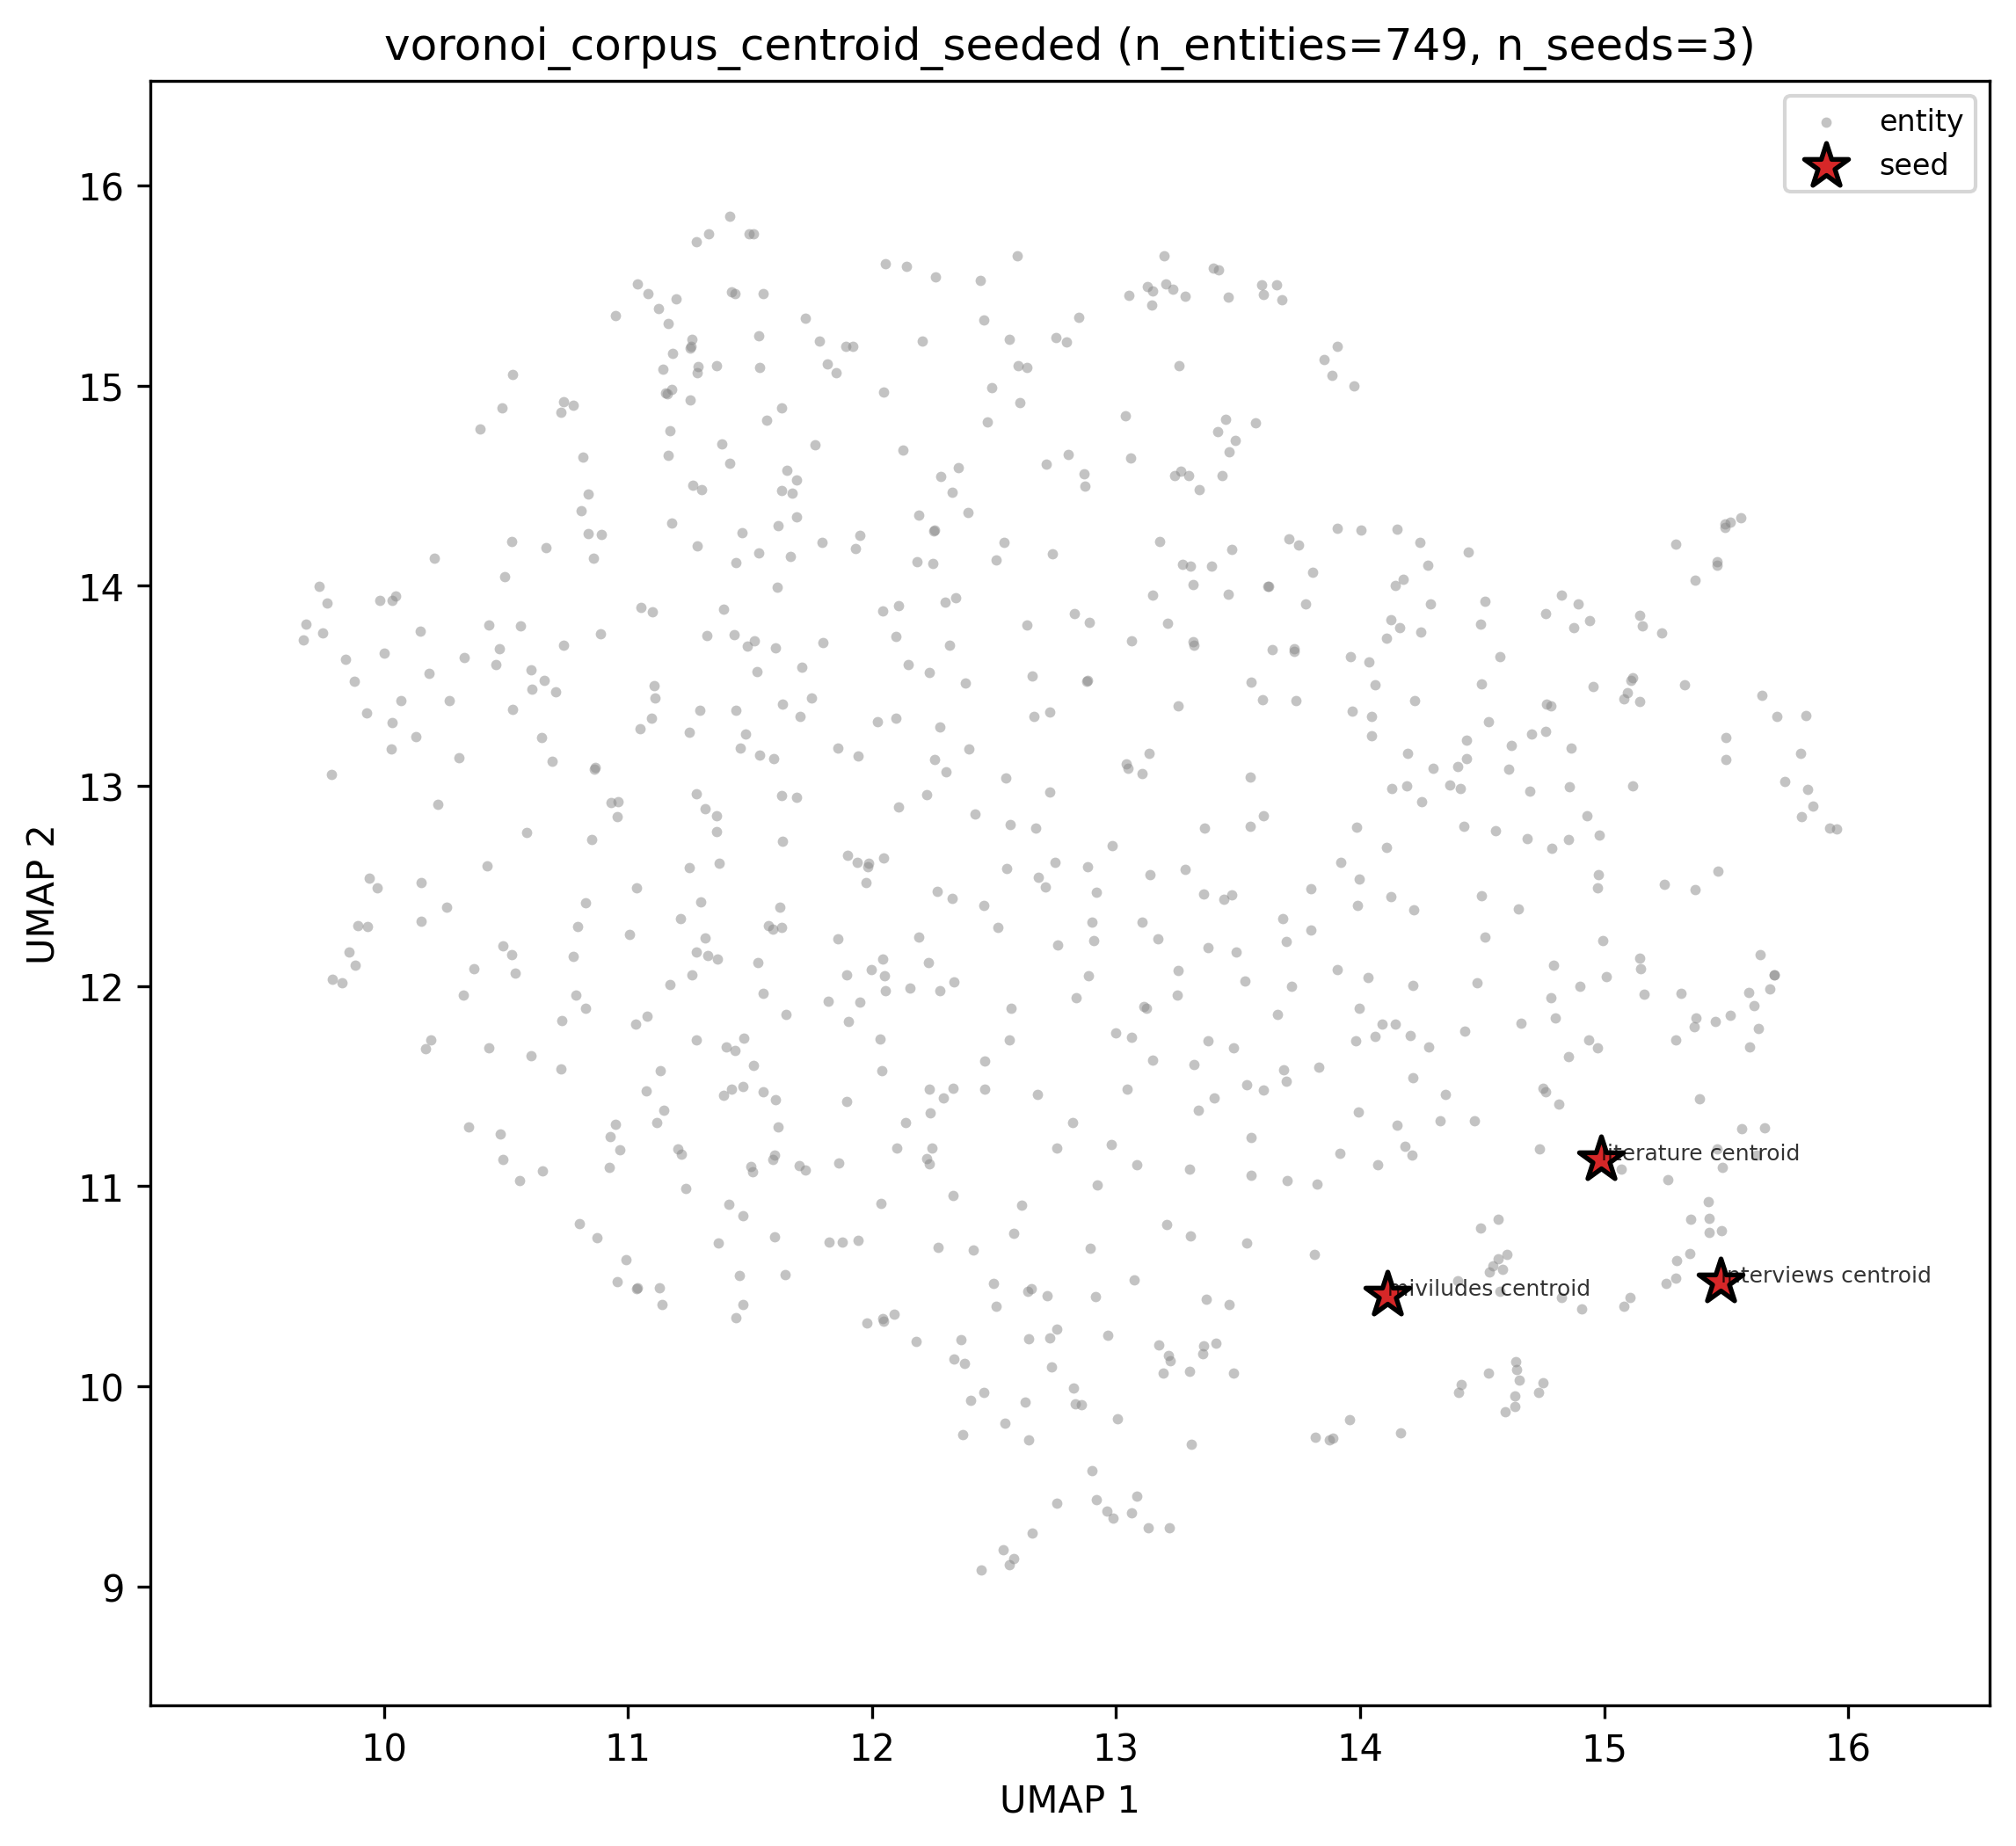
\includegraphics[width=0.75\textwidth]{figures/voronoi_corpus_centroid_seeded.png}
\caption{Corpus-centroid-seeded attempt -- only 3 seeds, no cell
boundaries drawn (scipy needs $\geq$4 points), this run.}
\label{fig:voronoi-corpus}
\end{figure}

% ============================================================
\section{What the rest of the toolkit found}
\label{sec:results}
% ============================================================

The remaining modules are materially unaffected by this run's entity-
layer fix (they concern expressions, not emergent entities); numbers
below are freshly computed against this run, not copied from the
previous report, and match it closely where nothing relevant changed.

\subsection{Free-listing rank audit}
Same verdict: \textbf{not usable}. Narrow check ("rank 1 is the
participant's own first claim"): \textbf{17/25} documents (68.0\%) --
down from the previous report's 18/25 because \texttt{b3-aug23-1213}'s
own rank-1 item is exactly the manually-excluded "Sept?" point
(Section~\ref{sec:spotcheck}), so it now correctly shows no valid
rank-1 item rather than one that happens to still pass the narrow check.
\texttt{response\_rank} plays no role anywhere else in this report.

\subsection{Global structure}
Selected pairwise centroid distances (full 8$\times$8 matrix in the
run's own CSV) -- essentially unchanged from the previous report:

\begin{table}[h!]
\centering
\small
\begin{tabular}{llrr}
\toprule
Source A & Source B & Euclidean & Cosine \\
\midrule
literature & miviludes & 8.00 & 0.50 \\
literature & interviews & 8.14 & 0.60 \\
miviludes & interviews & 12.00 & 0.22 \\
literature & miviludes\_criteria & 14.44 & 0.14 \\
miviludes & miviludes\_criteria & 12.10 & 0.51 \\
literature & emergent\_entities & 11.27 & 0.53 \\
\end{tabular}
\end{table}

\begin{figure}[h!]
\centering
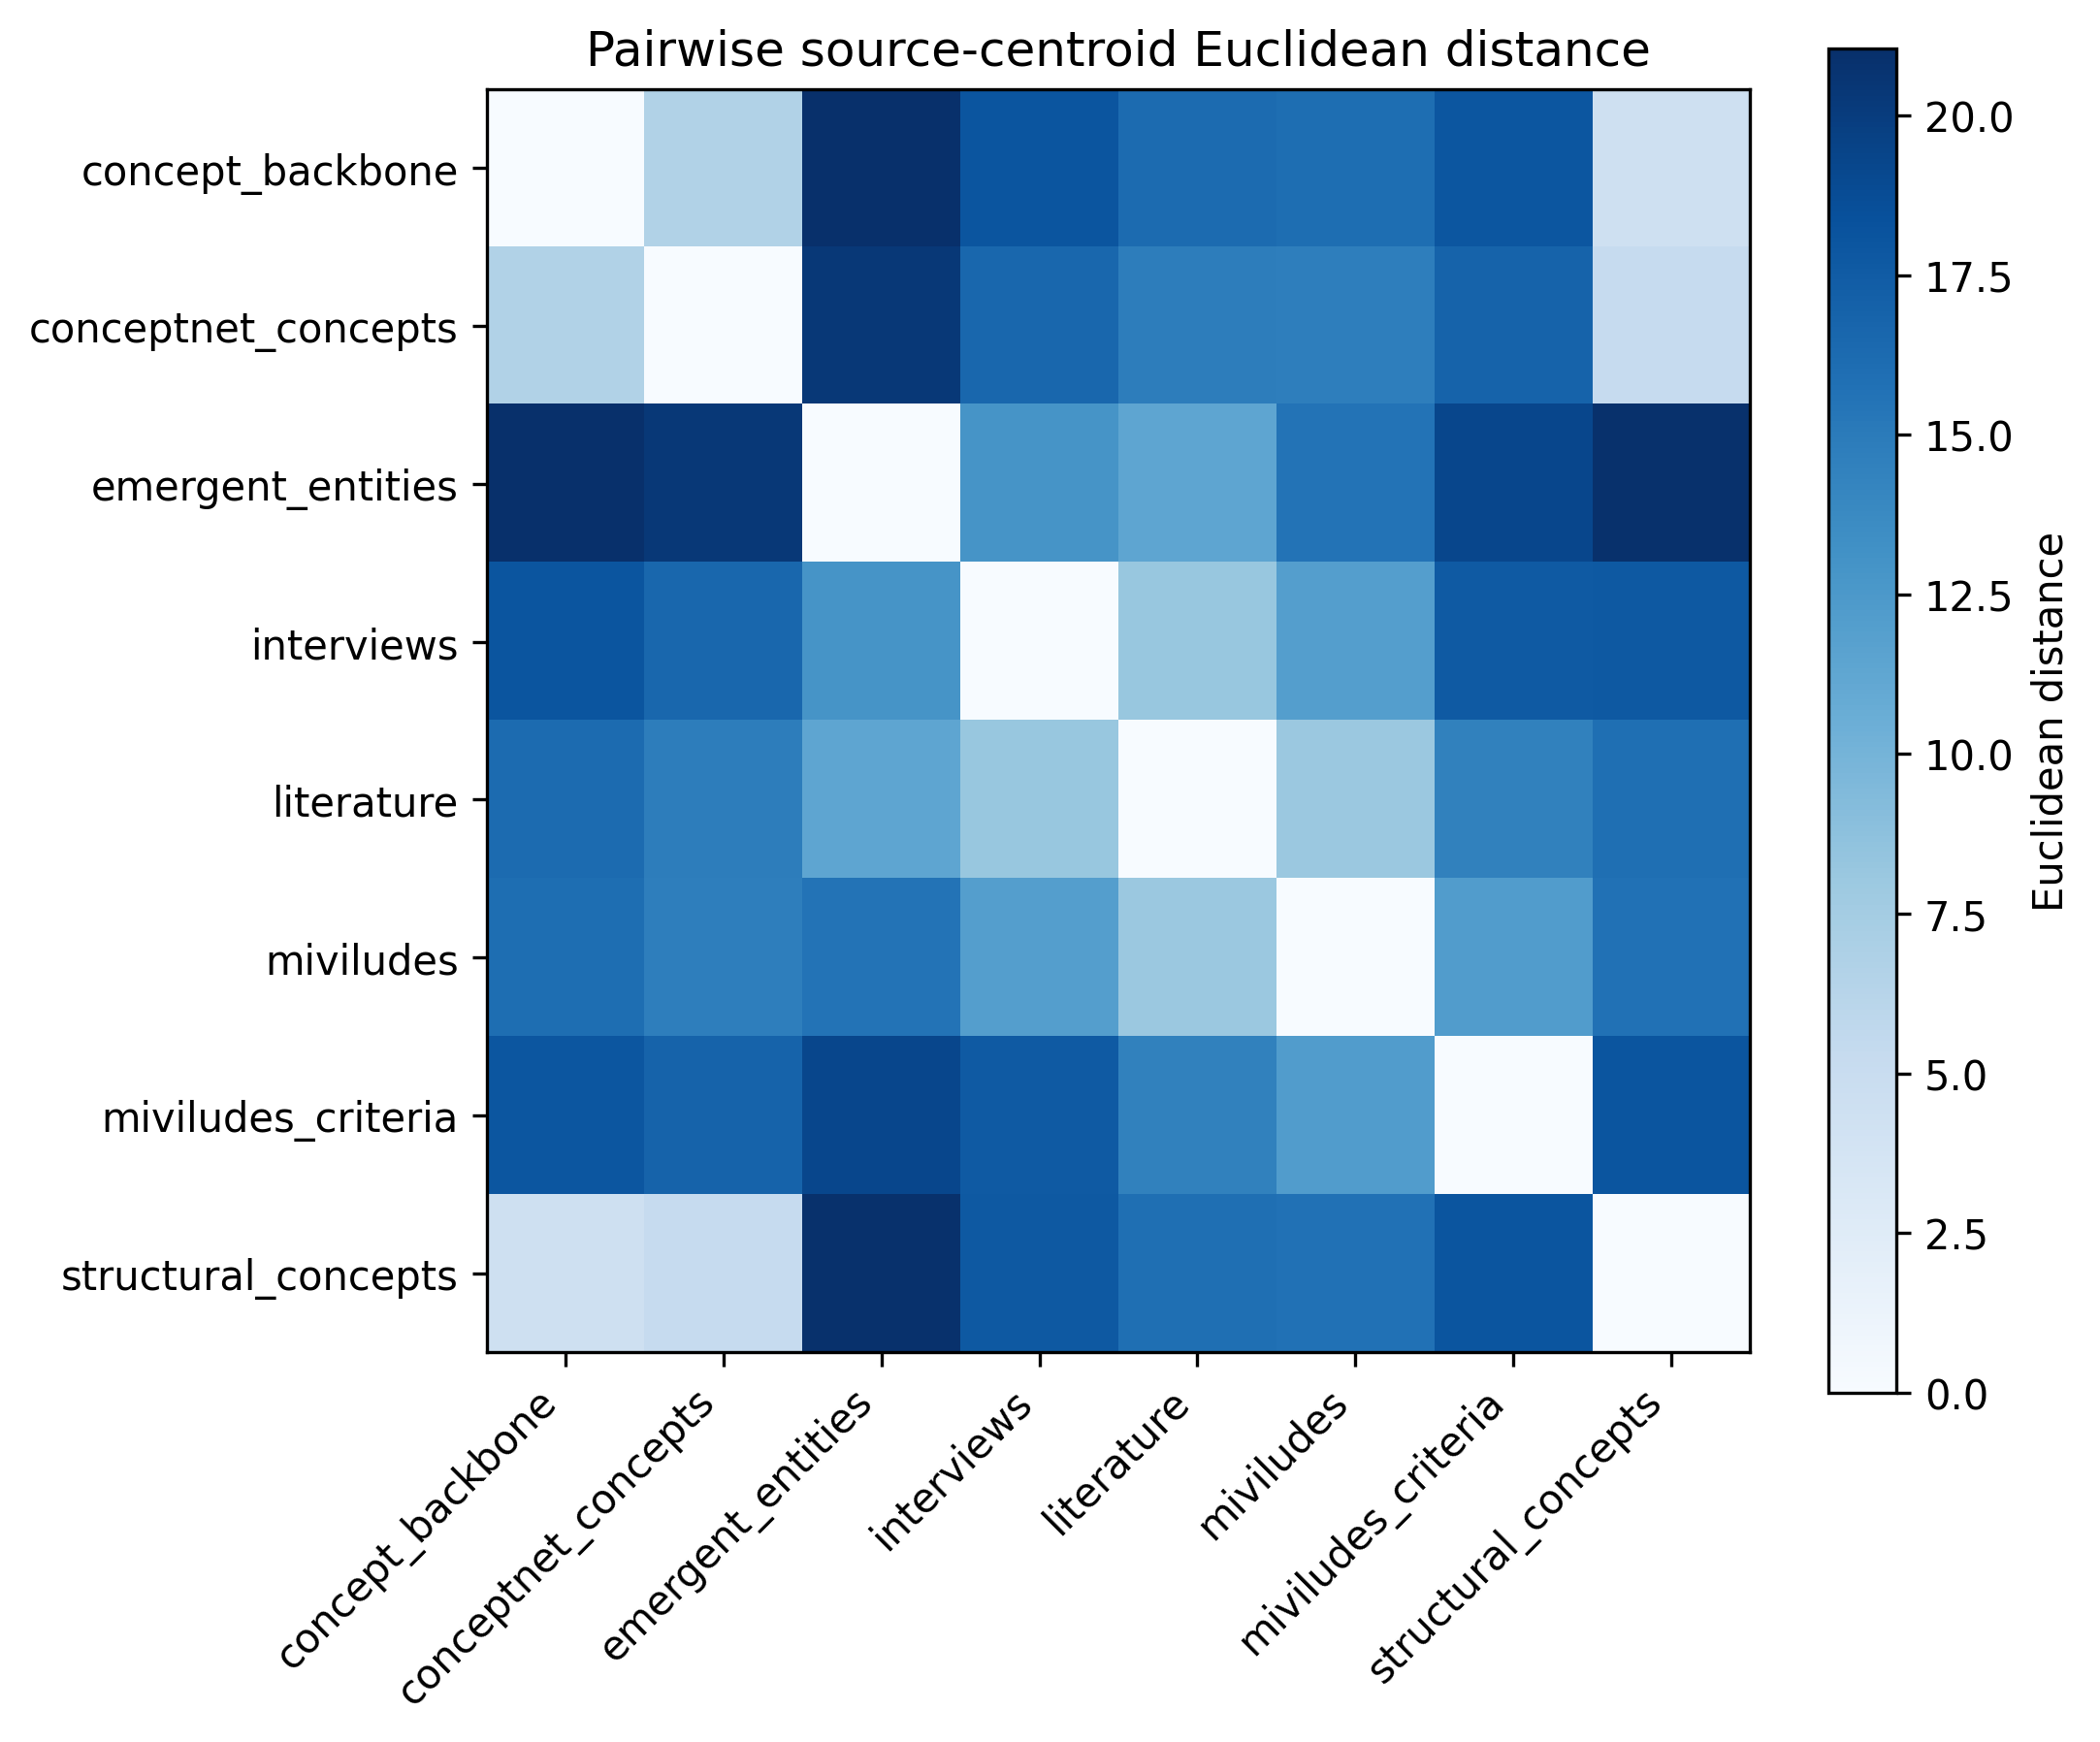
\includegraphics[width=0.85\textwidth]{figures/pairwise_source_centroid_heatmap.png}
\caption{Heatmap of pairwise centroid distances across all eight v2 sources, this run.}
\end{figure}

\subsection{Cluster structure}
Silhouette (equal-$n$, $k{=}10$): \textbf{0.0130} (95\% CI
[0.0098, 0.0164]) -- indistinguishable from the previous report's
0.0130. The three sources still overlap substantially rather than
forming separate clusters.

\begin{figure}[h!]
\centering
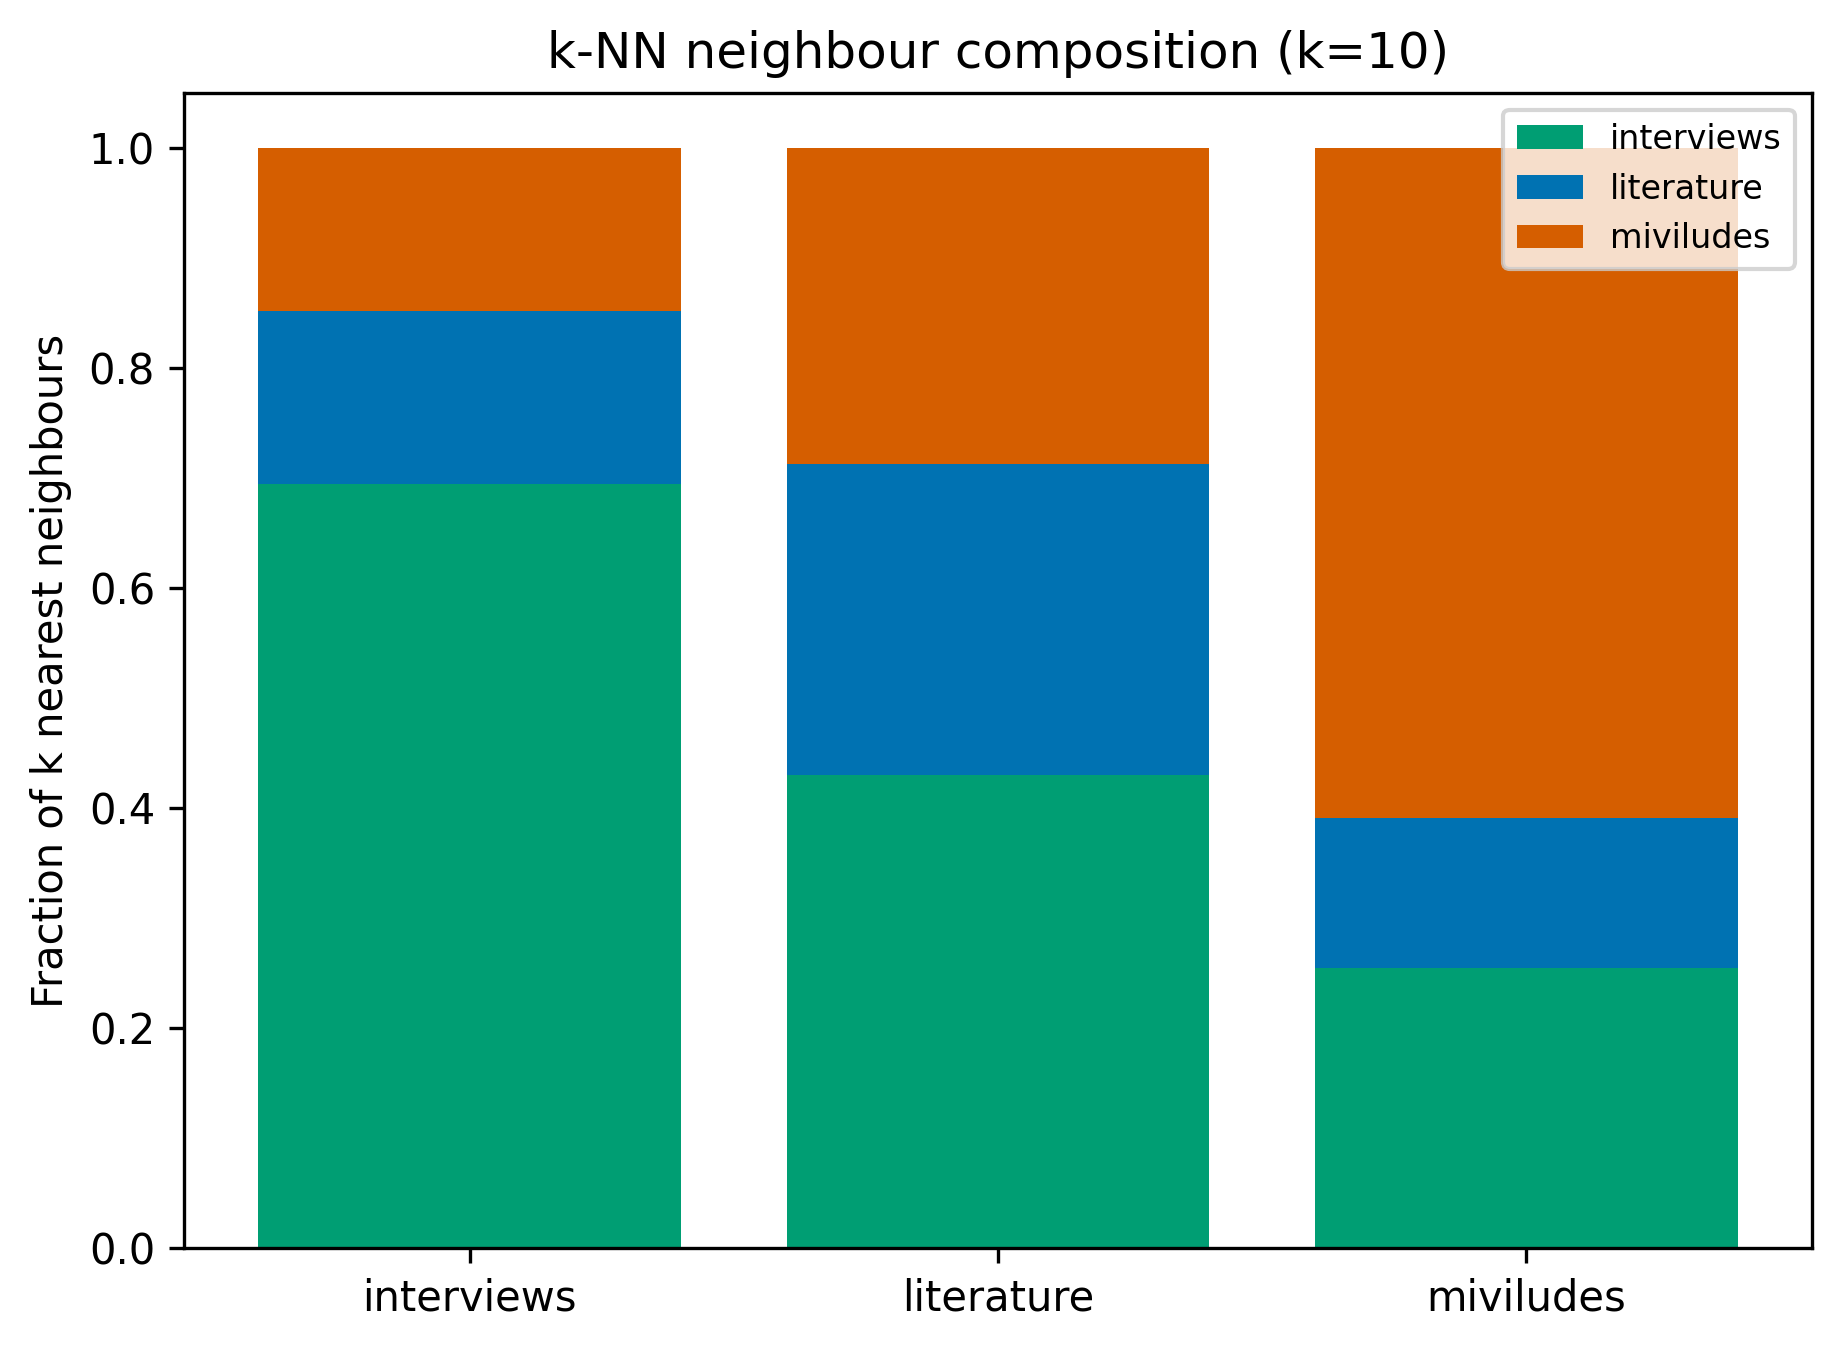
\includegraphics[width=0.85\textwidth]{figures/knn_composition_equal_n_k10.png}
\caption{k-NN neighbour composition at $k=10$, equal-$n$ sampling, this run.}
\end{figure}

\begin{figure}[h!]
\centering
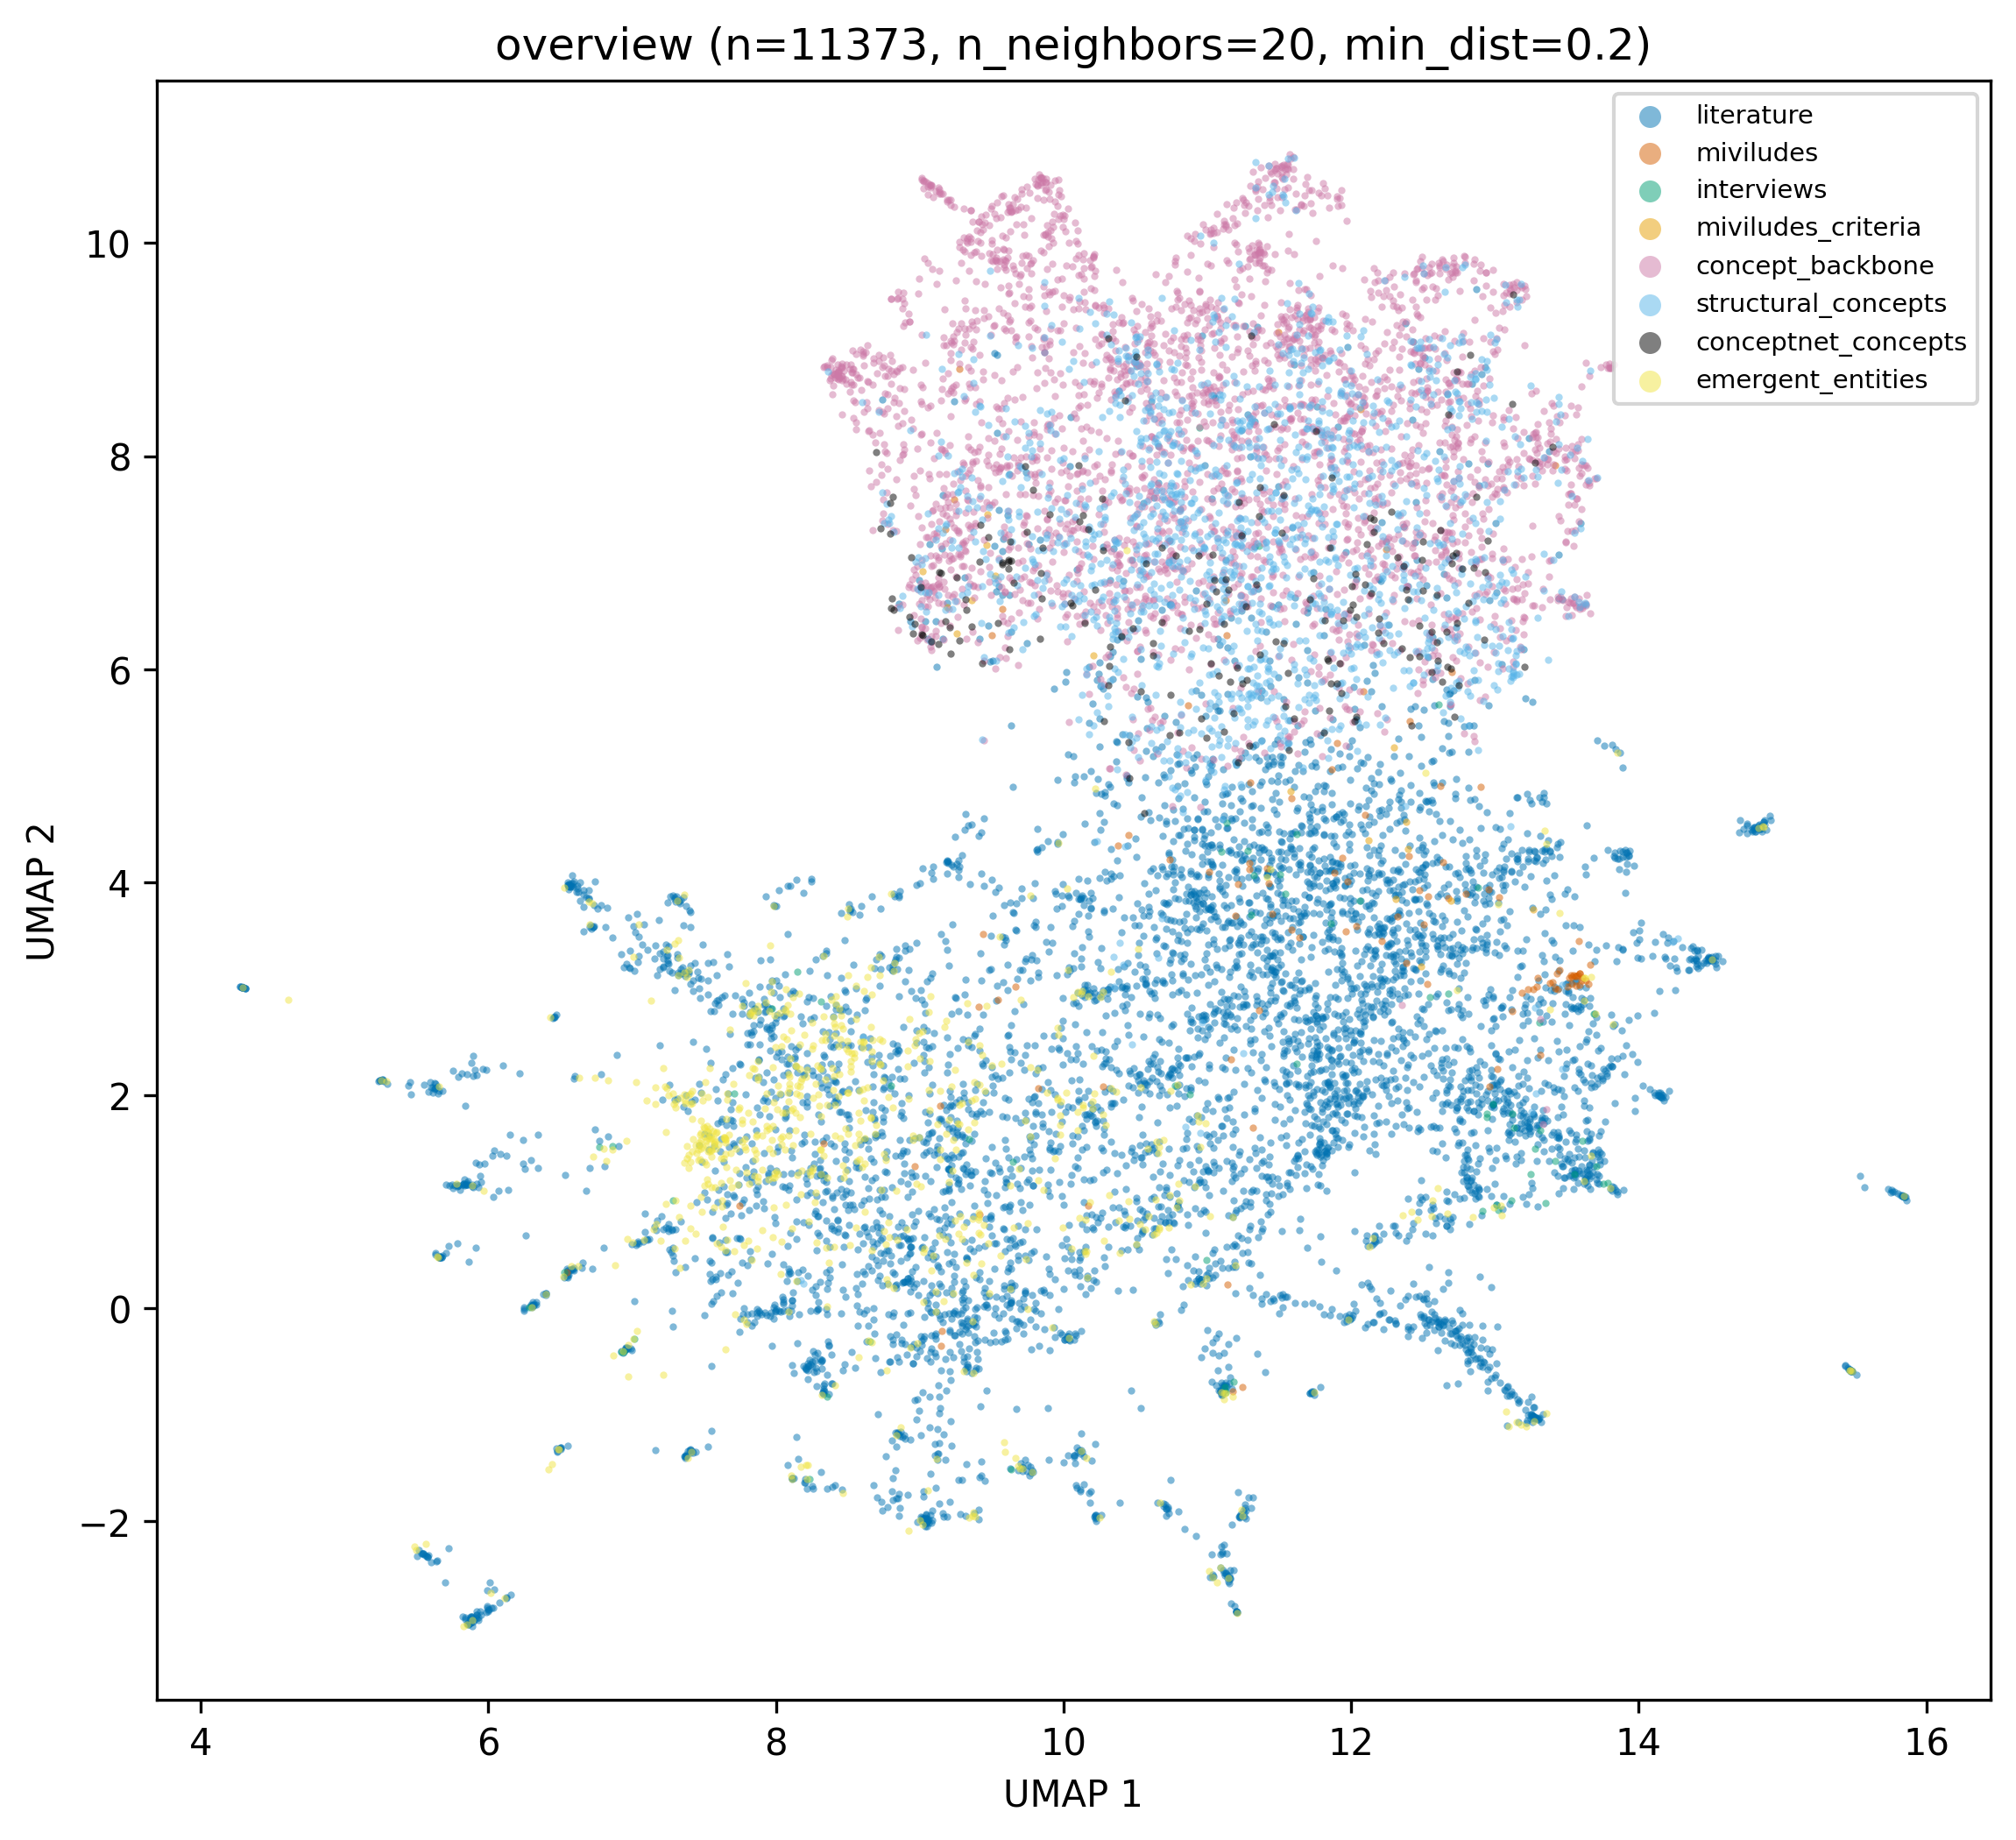
\includegraphics[width=0.85\textwidth]{figures/umap_overview_by_source_dataset_n20_d0.2.png}
\caption{Whole-space UMAP overview, coloured by source dataset, this run (11{,}373 points).}
\end{figure}

\subsection{Criterion neighbours}
Language-representation sensitivity: French-original vs.\ projected
English translation, \textbf{3 of 17} criteria change nearest corpus;
vs.\ raw cosine, \textbf{4 of 17} -- unchanged from the previous report.

\begin{figure}[h!]
\centering
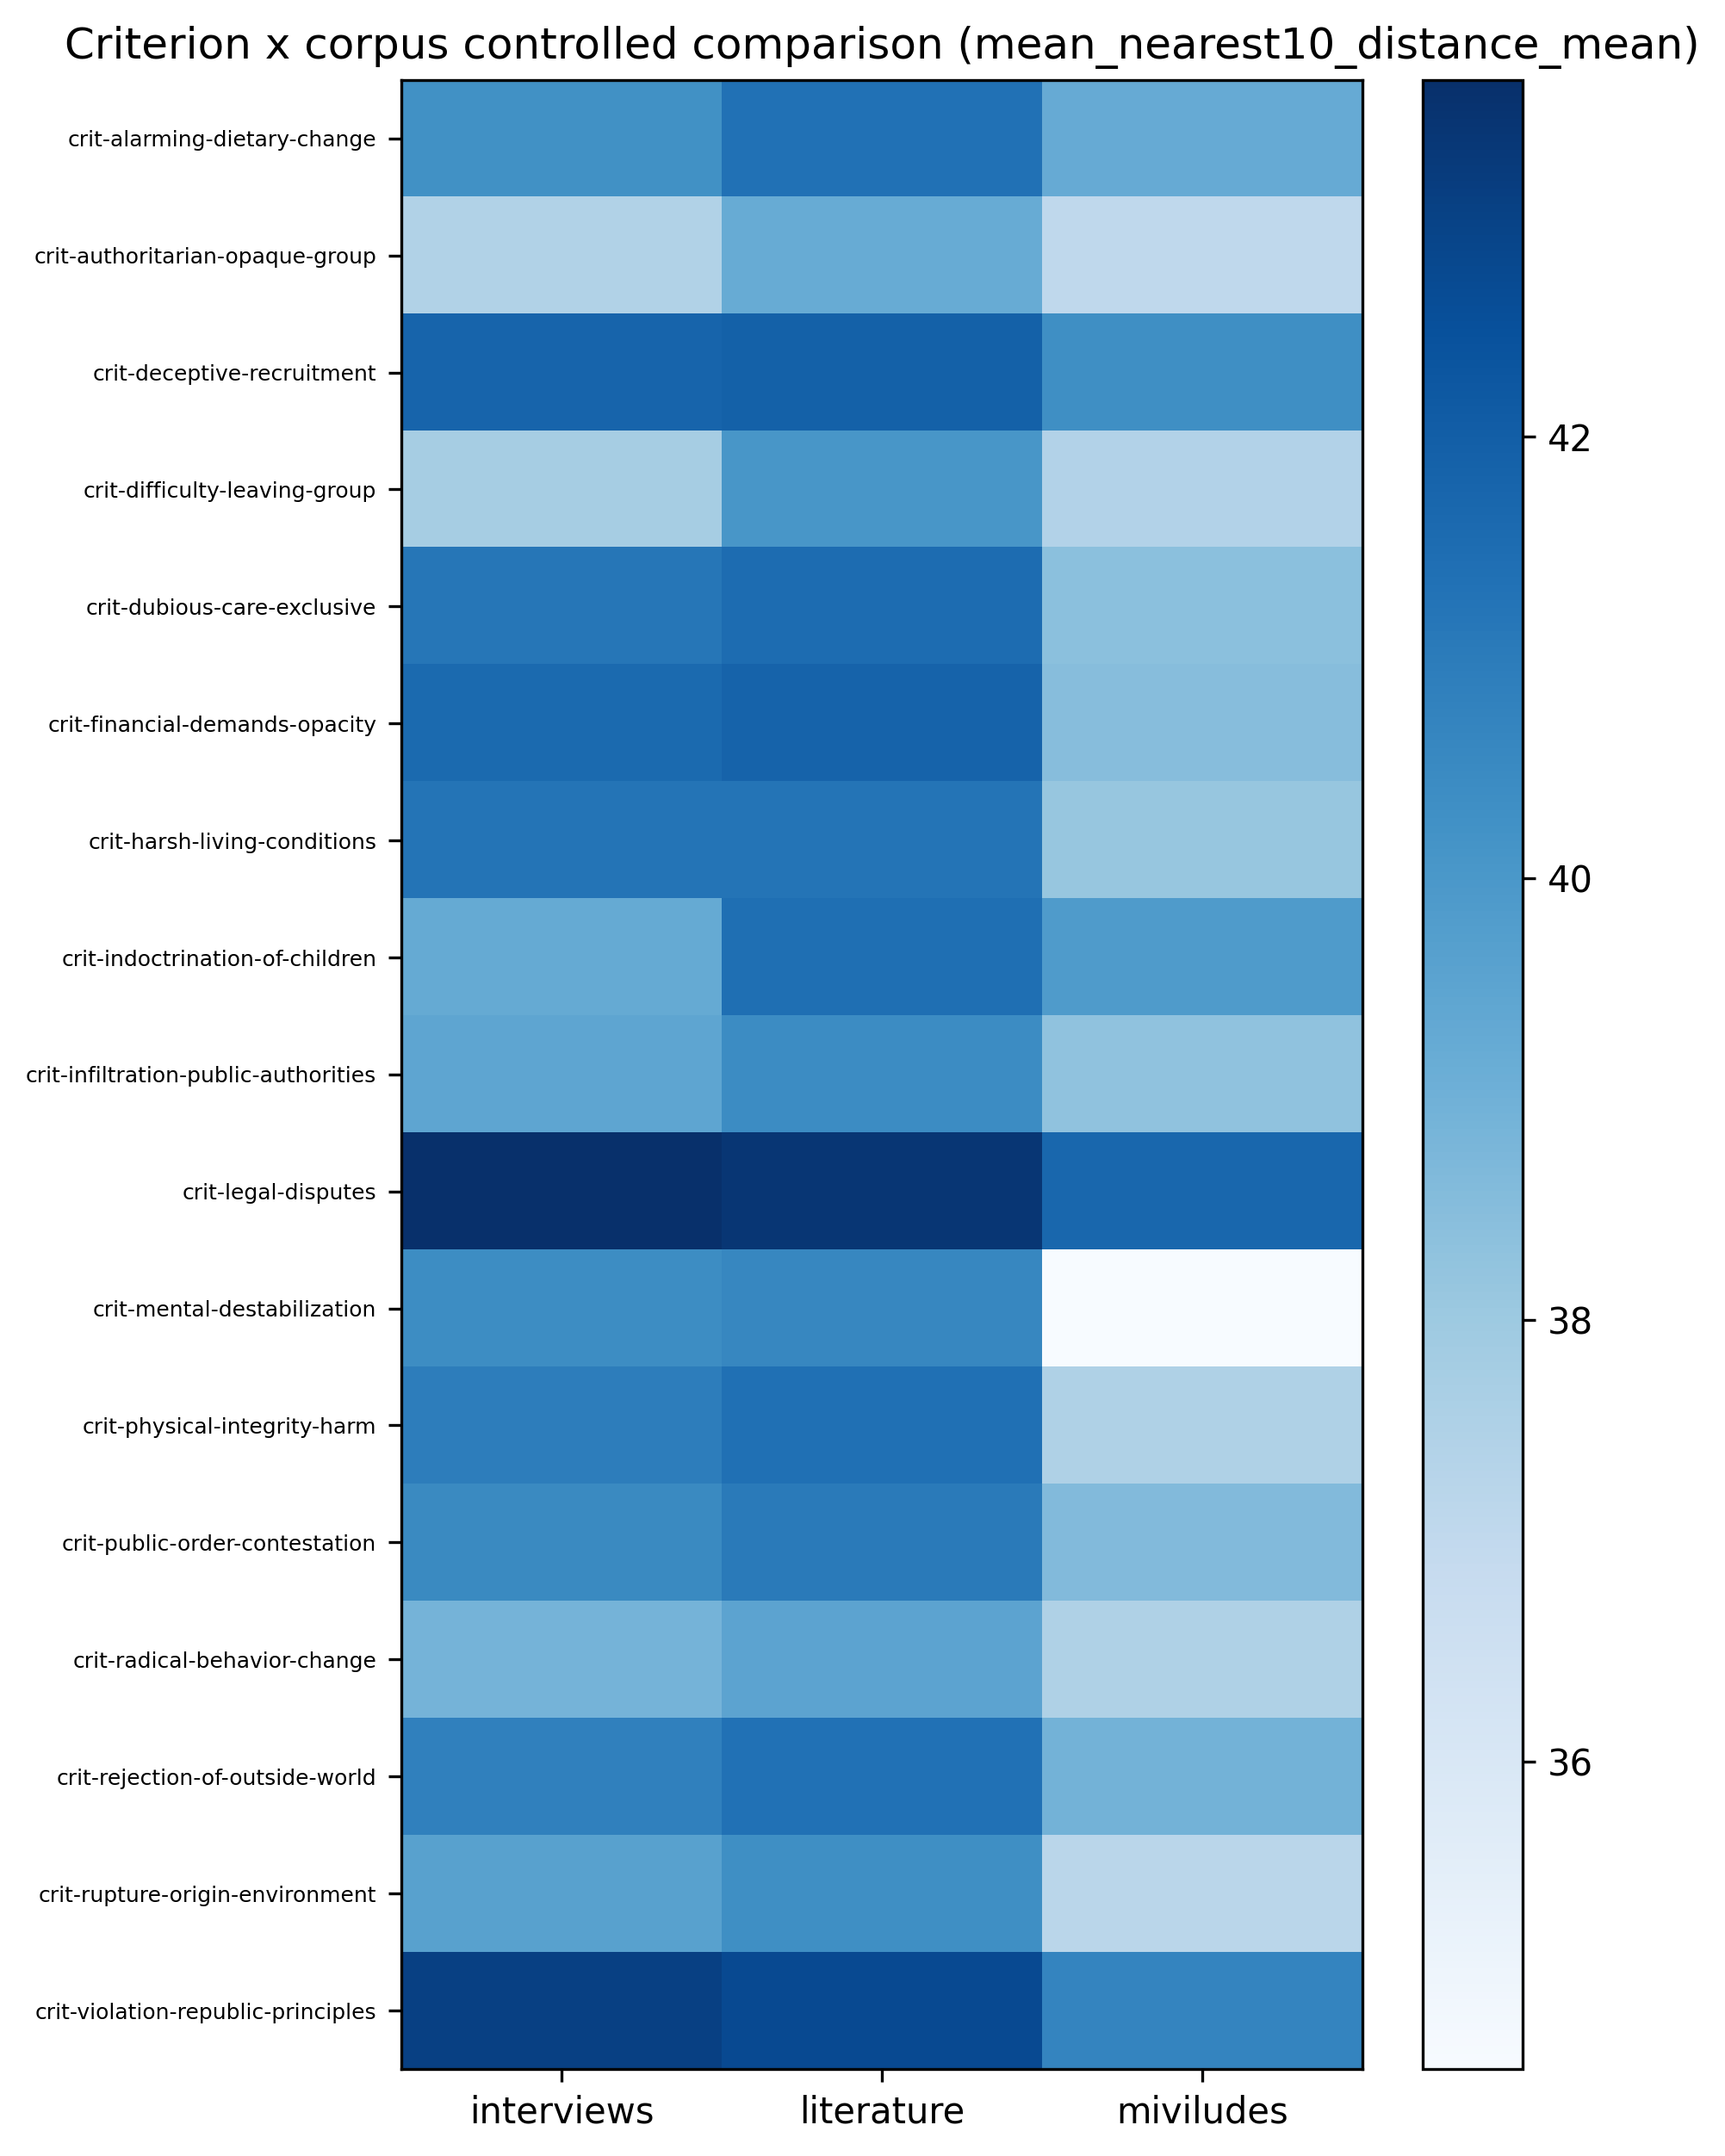
\includegraphics[width=0.85\textwidth]{figures/criterion_corpus_heatmap.png}
\caption{Heatmap of each of the 17 MIVILUDES criteria against the three expression corpora, this run.}
\end{figure}

One example of the per-criterion nearest-entity table (top-5 of 17,
unchanged from the previous report):

\begin{table}[h!]
\centering
\small
\begin{tabular}{ll}
\toprule
Rank & Nearest entity \\
\midrule
1 & thought reform and the psychology of totalism \\
2 & brainwashing \\
3 & ph\'enom\`ene d'emprise mentale \\
4 & silva mind control \\
5 & spiritism \\
\bottomrule
\end{tabular}
\caption{Nearest entities to \emph{crit-mental-destabilization}, this
run -- full 17-criterion table in
\texttt{analyze\_criterion\_neighbours/qualitative\_retrieval\_entities.csv}.}
\end{table}

\begin{table}[h!]
\centering
\begin{tabular}{ll}
\toprule
Corpus centroid & Rank 1 nearest entity \\
\midrule
literature & une secte. \\
miviludes & une secte. \\
interviews & une secte. \\
\bottomrule
\end{tabular}
\caption{Nearest entity to each of the 3 corpus centroids, this run --
unchanged: the generic French phrase "une secte." ranks \#1 for all
three, ahead of any specific named group.}
\end{table}

\subsection{Interview initial exemplars}
Unchanged: same 25 resolved/1 unavailable interviews, same
manually-verified quotes, re-measured against this run's space.

\begin{figure}[h!]
\centering
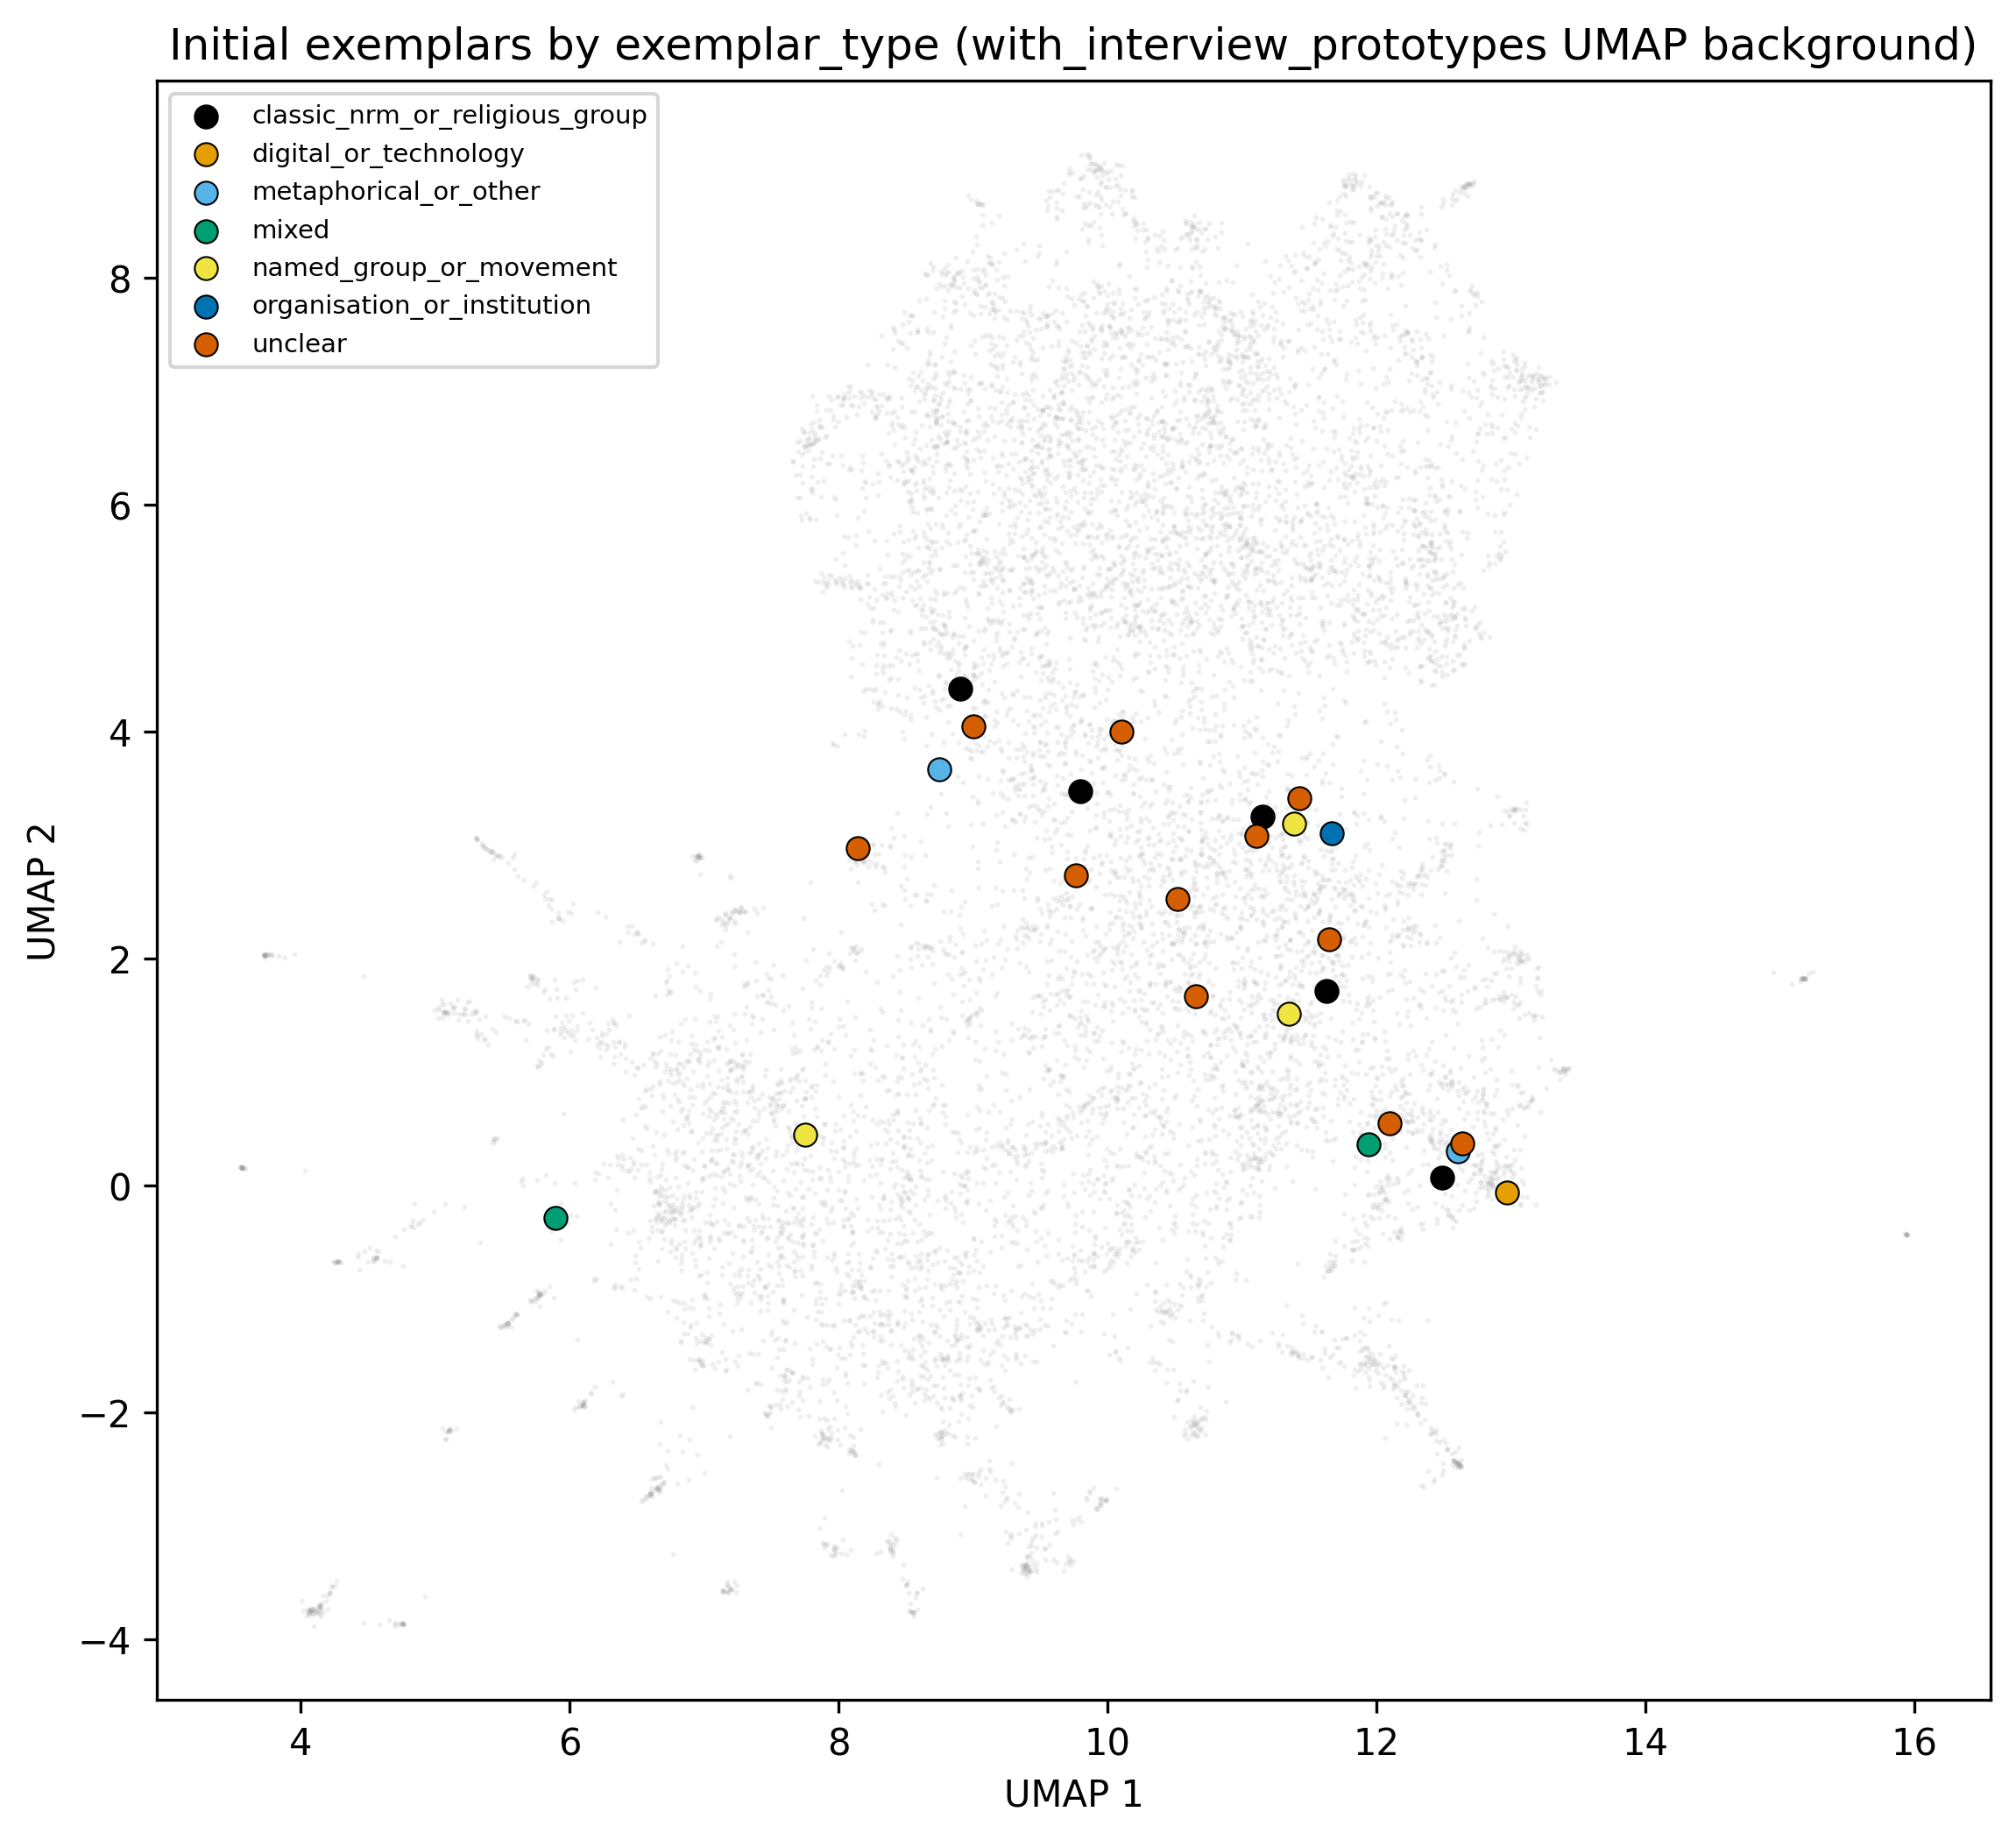
\includegraphics[width=0.75\textwidth]{figures/initial_exemplars_by_type.png}
\caption{Interview opening responses grouped by exemplar type, this run.}
\end{figure}

\subsection{Typicality and borderline points}
Unaffected by the entity fixes (concerns ordinary expressions). Same
pattern as before: the most atypical items per corpus are specific named
things (literature: "Jose Silva," "Asahara was born Matsumoto Chizuo in
1955"; miviludes: "Steiner-Waldorf schools," "Scientology"; interviews:
"Gourou," "Jehovah's Witnesses"), while the most typical are generic
statements ("This is Christianity.," "sectarian deviations," "the
cult").

\subsection{Focused projections}
23 curated populations generated this run, including the
\texttt{emergent\_entity\_focus} population (top 50 entities plus
overlay context):

\begin{figure}[h!]
\centering
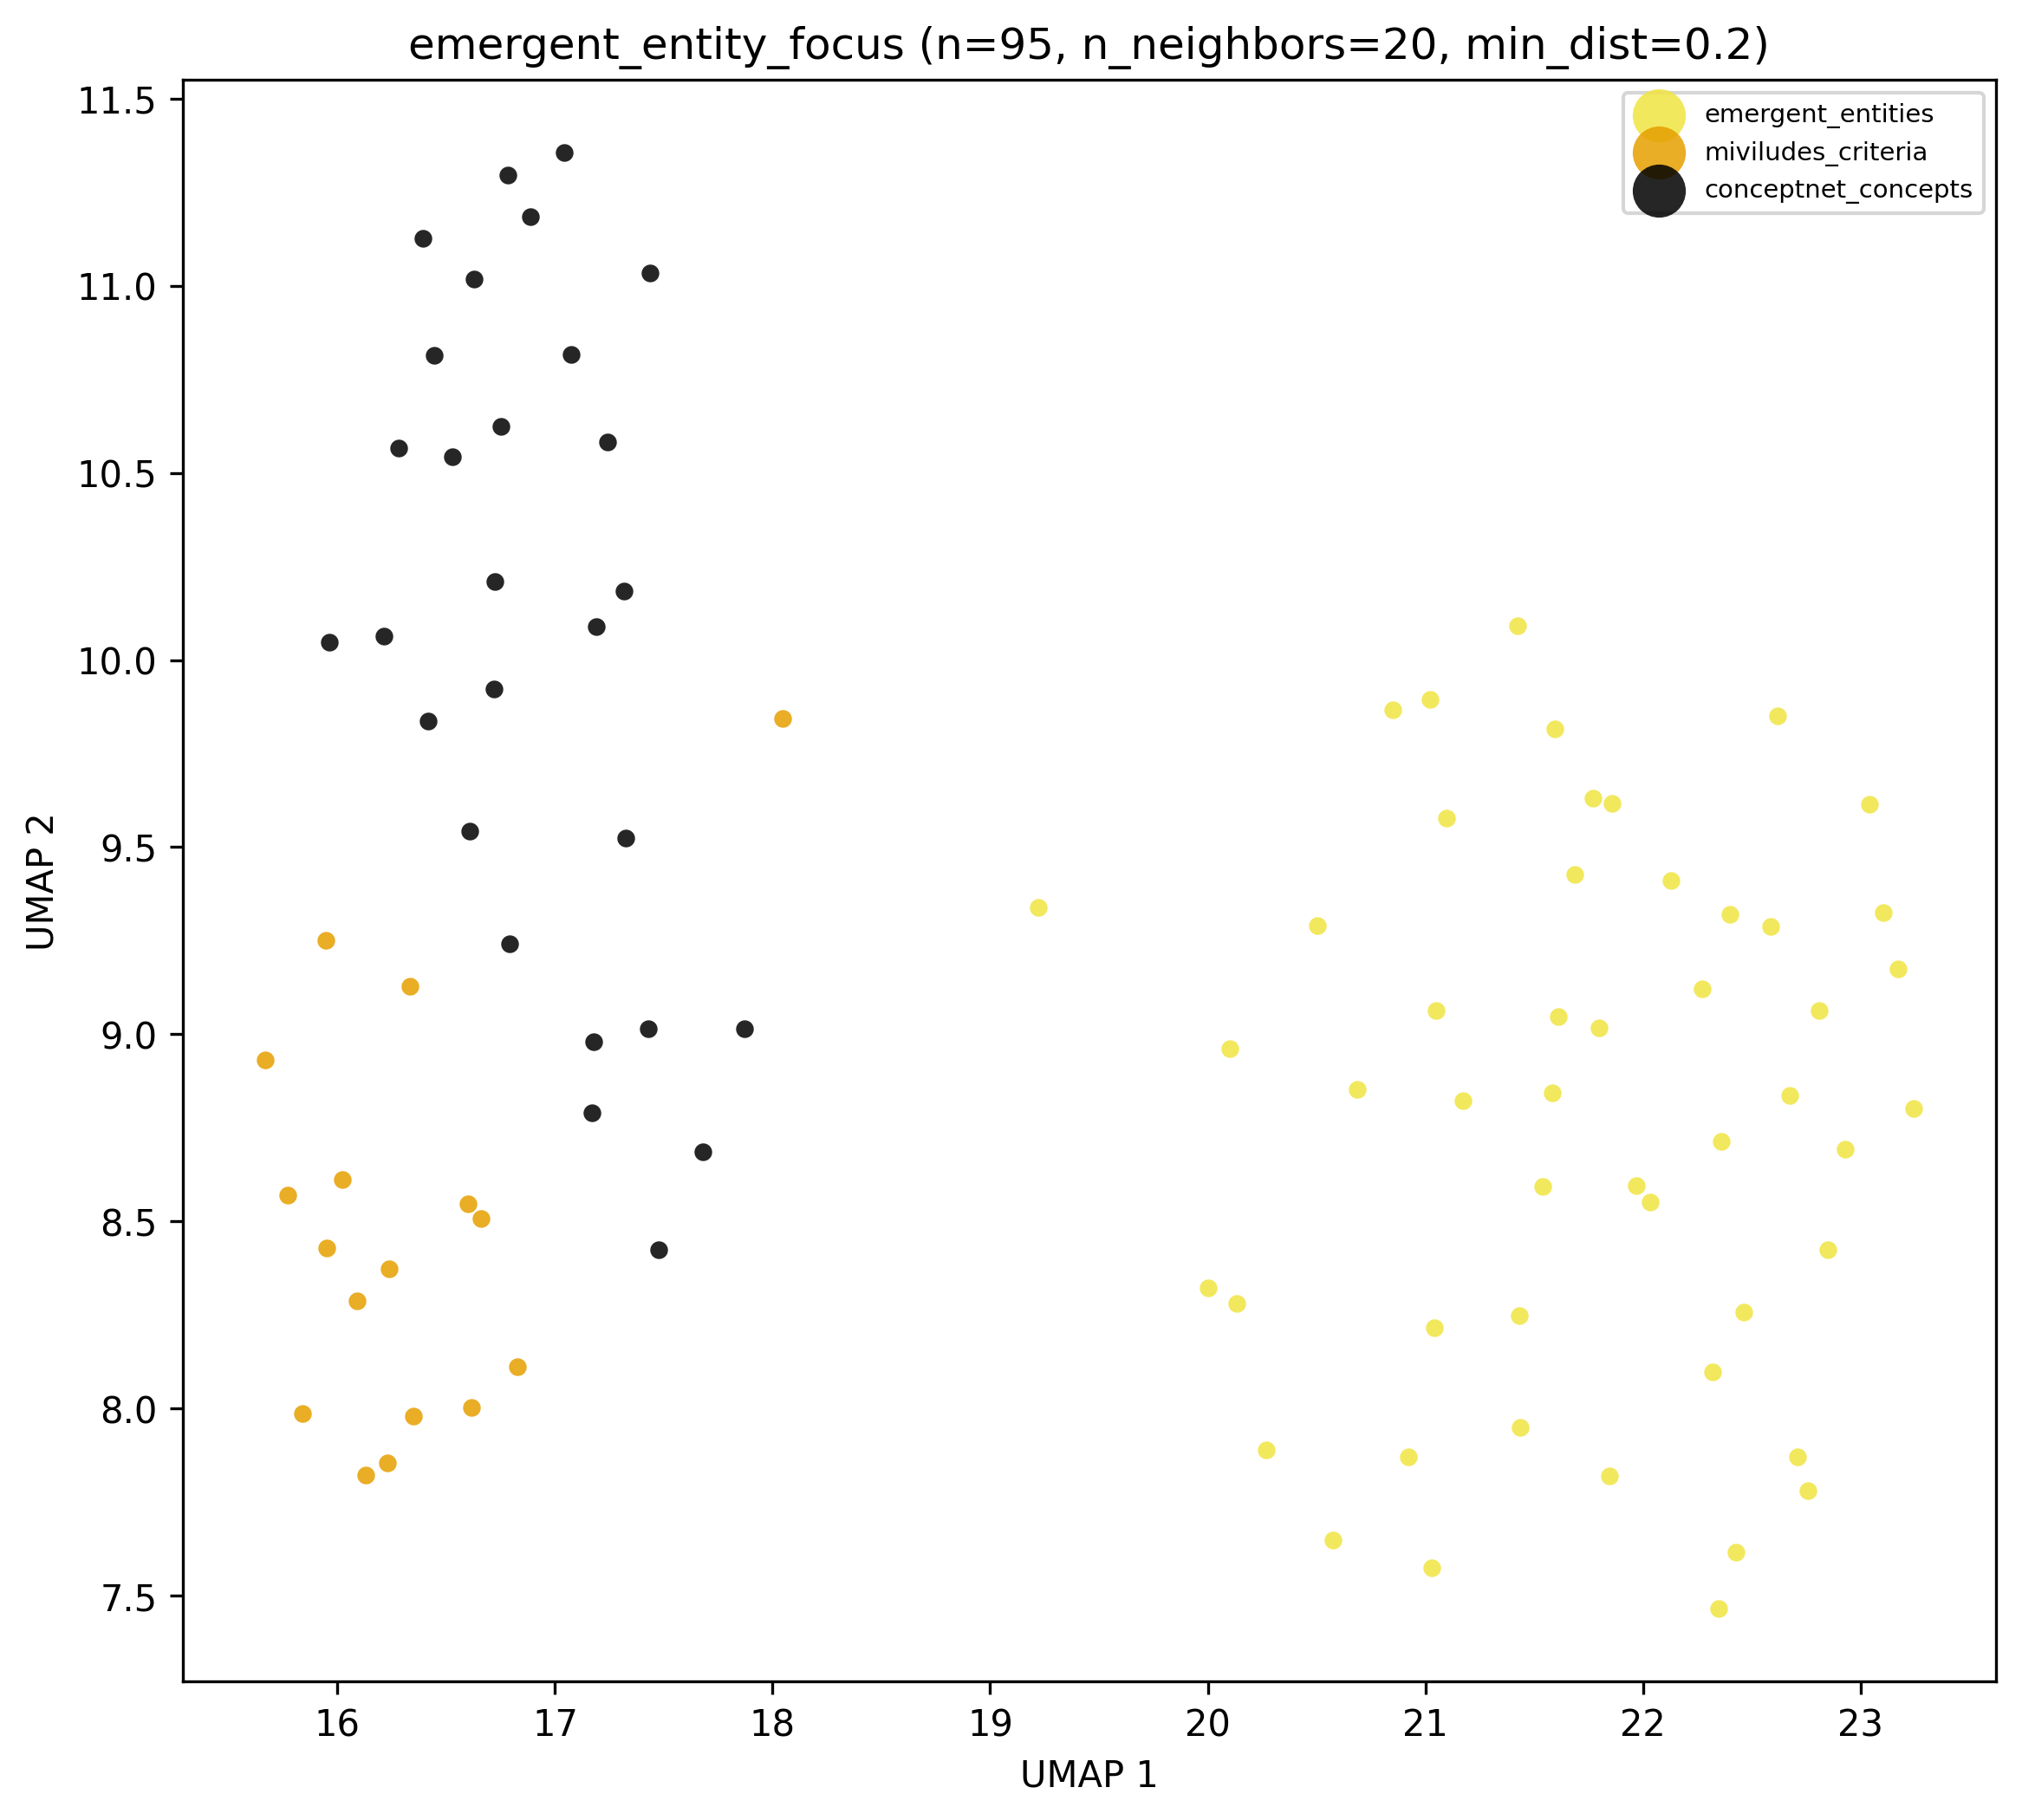
\includegraphics[width=0.8\textwidth]{figures/umap_emergent_entity_focus_by_source_dataset_n20_d0.2.png}
\caption{Focused UMAP of the top 50 emergent entities (plus neighbourhood context), coloured by source dataset, this run.}
\end{figure}

% ============================================================
\section{Publication-date effects (literature only)}
\label{sec:pubdate}
% ============================================================

Unaffected by this run's entity-layer fixes (literature-only, computed
directly from expression points). Year comes from each literature
\texttt{document\_id}; verified \textbf{5,741/5,741} (100\%) points have
an extractable year.

\begin{plainbox}[Governing principle]
A correlation or period-centroid shift here is a geometric fact about
extracted-expression embeddings by publication year; it is not, by
itself, evidence of a causal trend in scholarly opinion, a claim about
which period's literature is "more correct," or a claim that generalizes
beyond this specific 57-document sample.
\end{plainbox}

\textbf{Correlation}: Spearman rank correlation between publication year
and a point's distance to literature's own centroid: $\rho=-0.064$,
$p<0.0001$ (n=5,741) -- unchanged from the previous report. Weak effect,
statistically significant at this sample size.

\begin{figure}[h!]
\centering
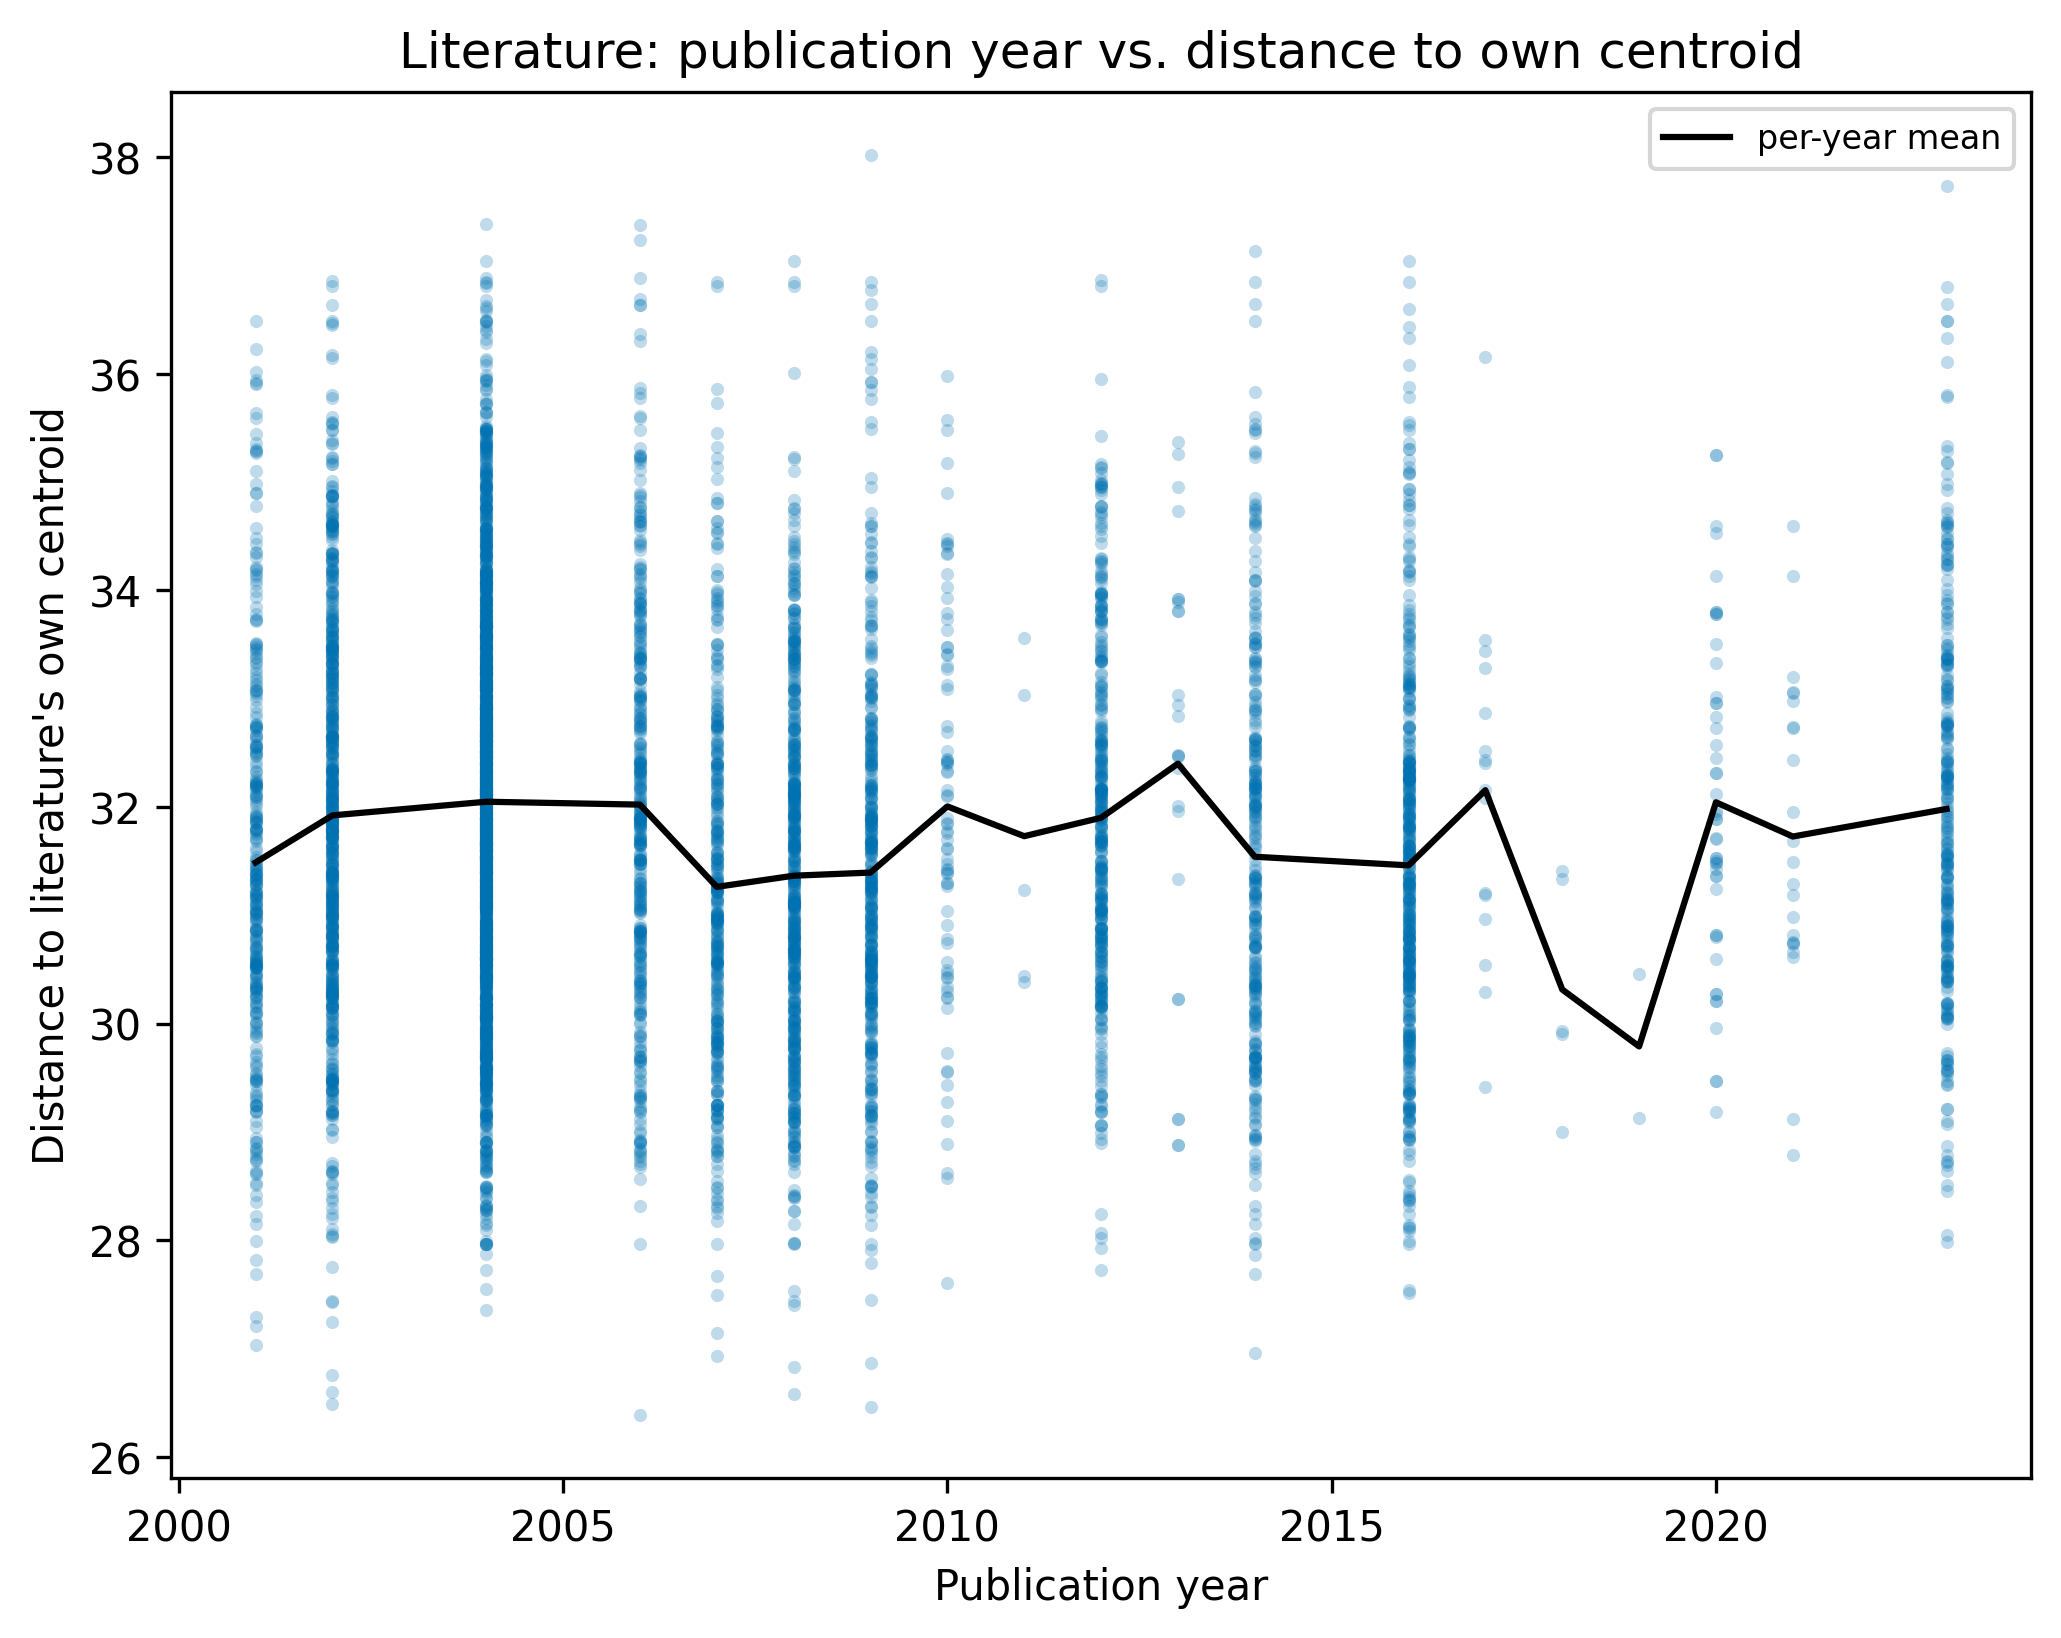
\includegraphics[width=0.75\textwidth]{figures/publication_year_vs_distance.png}
\caption{Literature: publication year vs.\ distance to literature's own
centroid, one point per expression, with the per-year mean overlaid, this run.}
\end{figure}

\textbf{Period drift}: early (2001--2004, n=2,556), mid (2006--2009,
n=1,634), late (2010--2023, n=1,551) -- unchanged split. The single
nearest MIVILUDES criterion to each period's own centroid is
\textbf{the same criterion in all three periods} -- \emph{Le changement
radical de comportement} ("radical behaviour change") -- distance
ranging 29.07--29.58 across the 2001--2023 span, unchanged from the
previous report.

% ============================================================
\section{Honesty notes -- what these numbers do not show}
\label{sec:honesty}
% ============================================================

\begin{itemize}[leftmargin=1.4em]
  \item \textbf{Corpus imbalance persists}: literature is 97.09\% of
  expression points; equal-$n$/equal-size corrections remain necessary
  and are used throughout.
  \item \textbf{Two entity-layer bugs are now fixed, but the underlying
  filters are still not a general citation detector.} A third residual
  gap remains, unchanged: externally-cited classical theorists who are
  not themselves among this corpus's own authors (e.g.\ Weber, Freud,
  Robert Jay Lifton) still pass, and this run's own cross-corpus cluster
  tables (Section~\ref{sec:crossgaps}) show at least one likely instance
  of it ("buxton; dixon; marlene dixon").
  \item \textbf{The epistemic-status breakdown currently answers very
  little}, not because the mechanism is broken but because 99.97\% of
  entity mentions come from a source field with no per-mention stance to
  report in the first place (Section~\ref{sec:epistemic}) -- a load-
  bearing limitation to keep in view before citing any
  "X entities are asserted/negated" claim from this layer.
  \item \textbf{The cross-corpus gap analysis does not itself decide
  what counts as a meaningful gap} -- raw distances only, no invented
  threshold, and at least two confounds (small corpus size mechanically
  inflating nearest-neighbour distances; residual cited-author noise)
  can produce a large distance without a genuine topical gap
  (Section~\ref{sec:crossgaps}).
  \item \textbf{French/English entity variants do not automatically
  merge.} "Scientology" (English) and "la scientologie" (French) are
  counted as separate entities unless the exact same string recurs -- so
  the 3 \texttt{shared\_all\_3} entities are a floor, not a ceiling, and
  the cross-corpus proximity check's "closest matches" this run were
  themselves mostly same-entity/different-wording pairs rather than
  genuinely distinct near-synonyms.
  \item \textbf{MIVILUDES is still two documents}, 108 expressions --
  its own independent clustering this run found only 2 clusters, one of
  them a 32-member catch-all mixing regulatory vocabulary with a handful
  of named groups.
  \item \textbf{The interview sample is a convenience sample}, 63 pooled
  expressions across 25 people.
  \item \textbf{\texttt{response\_rank} is still not usable} as a
  "first thing they thought of" signal.
  \item \textbf{2-D pictures are a reading aid, not evidence} --
  Section~\ref{sec:voronoi}'s criteria-seeded and corpus-centroid-seeded
  Voronoi diagrams still fail to render usefully, a UMAP out-of-sample
  artefact with no bearing on this document's high-dimensional retrieval
  elsewhere.
  \item \textbf{HDBSCAN leaves most entities (68\%, 512/749) as "noise"}
  at the threshold used -- expected for a heterogeneous set of named
  things, but a real limit on how much of the entity layer the
  cluster-based analyses actually speak to.
  \item \textbf{The publication-year terciles are size-imbalanced}
  (2,556/1,634/1,551 points) and \textbf{the year/distance correlation
  is real but very weak} ($\rho=-0.064$) -- a detectable but small
  effect, not "years matter a lot."
  \item \textbf{The per-interview QA trace (Section~\ref{sec:qa-trace})
  is a local sanity-check aid, not a reviewed research artefact} -- it
  surfaces exactly what the pipeline did, not whether every individual
  resolution is the "right" one; a manual read is still the researcher's
  own to do.
\end{itemize}

% ============================================================
\section{Possible interpretations}
\label{sec:interpretation}
% ============================================================

\begin{plainbox}[Read this box before the rest of this section]
Everything above this point is descriptive. Everything here is a
provisional \emph{reading} of that description, offered because it was
explicitly requested as a first pass -- not proof. Each is paired with a
reason it might be wrong.
\end{plainbox}

\begin{interpbox}[On the epistemic-status finding itself]
Finding that only 3 of 749 entities carry any known-stance mention is,
on one reading, itself informative about this project's current
extraction design: it shows that the richer, judge-verified
\texttt{entity\_anchors} field -- the only source with real per-mention
stance -- is a small minority contributor to total entity signal,
overwhelmingly outweighed by the broader, stance-blind
\texttt{domain\_terms} field. If entity-level stance tracking matters to
the thesis's argument, this suggests the leverage point is upstream (a
future extraction pass giving \texttt{domain\_terms} its own local
stance), not downstream in how the shared space pools what already
exists. \textbf{Why this might overstate the point}: it is also possible
that genuine negation/speculation about named entities is simply rare in
this corpus regardless of extraction field -- flat assertion ("X is a
cult") may just be the dominant rhetorical mode when a text names a
specific group at all, in which case a richer stance-tagging pass would
still find mostly "asserted," not a hidden reservoir of negated/
speculative mentions. This run's data cannot distinguish "the field
can't see it" from "there isn't much of it to see."
\end{interpbox}

\begin{interpbox}[On the cross-corpus gap findings]
The heavier check's clearest pattern -- literature's most historically
notorious named groups (Manson Family, Peoples Temple, Clapham Sect)
sitting farthest from any MIVILUDES entity, while more \emph{currently
salient} or \emph{culturally visible} groups (Scientology, Moonies,
Mormons) sit close to both MIVILUDES and interview vocabulary -- is
consistent with a reading that MIVILUDES's institutional
sectarian-drift framework, being an ongoing regulatory-monitoring
document, orients toward groups perceived as live administrative/legal
concerns rather than a historical register of every notorious case
academic literature discusses. \textbf{Why this might be wrong}:
MIVILUDES is only 2 documents and 108 expressions -- its own clustering
found just 2 clusters total, meaning "nearest MIVILUDES entity" for
\emph{any} literature cluster is drawn from an unusually small,
low-resolution population; a much larger MIVILUDES corpus might turn out
to mention the Manson Family or Peoples Temple by name after all, simply
never having had the raw text volume for that mention to survive
extraction and clustering at the thresholds used here.
\end{interpbox}

\begin{interpbox}[On the lightweight check's near-total MIVILUDES/interview absence from literature-heavy clusters]
40 of 49 unified clusters have zero MIVILUDES presence and 28 have zero
interview presence, while literature is present everywhere. One
reading: this simply restates corpus size (literature: 5,741
expressions; MIVILUDES: 108; interviews: 64) in geometric form, and
should not by itself be read as MIVILUDES or interviewees having
"nothing to say" about most of the entity space -- a corpus with 50x
fewer expressions will mechanically produce far fewer qualifying
entities regardless of topical breadth. \textbf{Why this reading is
probably right, and worth stating plainly}: the heavier check's own
per-corpus thresholds already account for this asymmetry (interviews
qualifies an entity at just 1 mention, vs.\ literature's 10), and even
so interviews' own 107 qualifying entities are a small fraction of
literature's 667 -- the corpus-size explanation is not a stretch here,
it is close to the whole story, and any Results-chapter framing of these
absence counts should lead with that rather than imply a topical claim
the numbers alone do not support.
\end{interpbox}

\begin{interpbox}[On what the second entity-layer bug shows about the first]
That a second, independent bug in the same stop-list mechanism survived
the previous report's own verification (checking whether known scholar
names appeared in a top-20/30-by-mention list, which they never would
regardless of whether the stop-list worked) is itself a small
methodological lesson: a verification check can pass while testing the
wrong thing. \textbf{Why this might overstate the point}: the bug was
still found and fixed within the same research process, via a different
downstream check (the cross-corpus clustering module) rather than an
external audit -- arguably evidence the project's overall practice of
building multiple independent views onto the same data (lightweight and
heavy gap checks, in this instance) is doing real verification work,
not evidence the verification discipline itself is unreliable.
\end{interpbox}

% ============================================================
\section{Using this document to write the Results chapter}
% ============================================================

Sections~\ref{sec:epistemic} and~\ref{sec:crossgaps} are new this run
and, per explicit researcher feedback, are written to foreground
findings and concrete example tables rather than methodology narrative
-- the fixes and mechanisms behind them are documented once, in
\texttt{thesis/03\_Content/3\_Methods.tex}, not repeated here.
Section~\ref{sec:entities}'s green fixbox is the one exception, kept
because the correction itself (a second, independently-found bug in the
same stop-list mechanism) is a methodologically relevant fact about how
much scrutiny an automated "count of named things" deserves, consistent
with how the first such fix was treated in the previous report.
Section~\ref{sec:qa-trace} documents a QA aid that exists to let the
researcher independently confirm the numbers above are trustworthy
before they are cited -- doing that check is still the researcher's own
next step, not something this document can substitute for.
Section~\ref{sec:interpretation} remains a first, provisional pass, kept
structurally separate from descriptive fact throughout, offered as a
starting point for argument, not a finished answer.

\end{document}
